\documentclass{article}\usepackage[]{graphicx}\usepackage[]{color}
% maxwidth is the original width if it is less than linewidth
% otherwise use linewidth (to make sure the graphics do not exceed the margin)
\makeatletter
\def\maxwidth{ %
  \ifdim\Gin@nat@width>\linewidth
    \linewidth
  \else
    \Gin@nat@width
  \fi
}
\makeatother

\definecolor{fgcolor}{rgb}{0.345, 0.345, 0.345}
\newcommand{\hlnum}[1]{\textcolor[rgb]{0.686,0.059,0.569}{#1}}%
\newcommand{\hlstr}[1]{\textcolor[rgb]{0.192,0.494,0.8}{#1}}%
\newcommand{\hlcom}[1]{\textcolor[rgb]{0.678,0.584,0.686}{\textit{#1}}}%
\newcommand{\hlopt}[1]{\textcolor[rgb]{0,0,0}{#1}}%
\newcommand{\hlstd}[1]{\textcolor[rgb]{0.345,0.345,0.345}{#1}}%
\newcommand{\hlkwa}[1]{\textcolor[rgb]{0.161,0.373,0.58}{\textbf{#1}}}%
\newcommand{\hlkwb}[1]{\textcolor[rgb]{0.69,0.353,0.396}{#1}}%
\newcommand{\hlkwc}[1]{\textcolor[rgb]{0.333,0.667,0.333}{#1}}%
\newcommand{\hlkwd}[1]{\textcolor[rgb]{0.737,0.353,0.396}{\textbf{#1}}}%
\let\hlipl\hlkwb

\usepackage{framed}
\makeatletter
\newenvironment{kframe}{%
 \def\at@end@of@kframe{}%
 \ifinner\ifhmode%
  \def\at@end@of@kframe{\end{minipage}}%
  \begin{minipage}{\columnwidth}%
 \fi\fi%
 \def\FrameCommand##1{\hskip\@totalleftmargin \hskip-\fboxsep
 \colorbox{shadecolor}{##1}\hskip-\fboxsep
     % There is no \\@totalrightmargin, so:
     \hskip-\linewidth \hskip-\@totalleftmargin \hskip\columnwidth}%
 \MakeFramed {\advance\hsize-\width
   \@totalleftmargin\z@ \linewidth\hsize
   \@setminipage}}%
 {\par\unskip\endMakeFramed%
 \at@end@of@kframe}
\makeatother

\definecolor{shadecolor}{rgb}{.97, .97, .97}
\definecolor{messagecolor}{rgb}{0, 0, 0}
\definecolor{warningcolor}{rgb}{1, 0, 1}
\definecolor{errorcolor}{rgb}{1, 0, 0}
\newenvironment{knitrout}{}{} % an empty environment to be redefined in TeX

\usepackage{alltt}
\usepackage[utf8]{inputenc}
\usepackage[portuguese]{babel}
\usepackage[backend=bibtex,style=alphabetic,citestyle=authoryear]{biblatex}
\bibliography{ref.bib}
\usepackage{float}
\usepackage{graphicx}

\author{Bernardo Paulsen \\ Matheus Bragagnolo}
\title{Prova 2 - Estatística Econômica Aplicada}
\date{ }
\IfFileExists{upquote.sty}{\usepackage{upquote}}{}
\begin{document}

\maketitle

\tableofcontents


\section{Introdução}

    O objetivo do presente trabalho é analisar uma série temporal univariada utilizando os métodos apresentados na cadeira ECOP124 (Estatística Econômica Aplicada) ministrada pelos professores Carlos Schonerwald e Fernando Sabino. O trabalho será baseado nos tópicos:
    
    \begin{itemize}
        \item Pontos de Mudança e Quebras Estruturais;
        \item Modelos ARMA Univariados;
        \item Mais Testes e Previsões;
        \item Não Estacionariedade, Testes de Raiz Unitária e Modelos ARIMA(p,d,q);
        \item Modelos de Volatilidade Univariada.
    \end{itemize}
    
    Como material de apoio para o desenvolvimento do trabalho encontram-se disponíveis notas de aula e vídeo-aulas. Este trabalho é referente à dupla 1, à qual coube a subsérie temporal 4 (observações 5775 à 6564). O código do trabalho pode ser encontrado em repositório do github no link: https://github.com/bernardopaulsen/ecop124.


\section{Preparatórios}

    \subsection{Importação de Bibliotecas}

        Primeriamente, precisamos importar as bibliotecas que serão necessárias para executar os códigos das próximas seções. Utilizamos as seguintes bibliotecas:
    
        \begin{itemize}
            \item \textit{astsa} (\cite{astsa}): função \textit{sarima}.
            \item \textit{DescTools} (\cite{desctools}): função \textit{TheilU};
            \item \textit{forecast} (\cite{forecast}): função \textit{accuracy};
            \item \textit{lubridate} (\cite{lubridate}): função \textit{parse\underline{ }date\underline{ }time};
            \item \textit{notsTest} (\cite{nortstest}): função \textit{Lm.test};
            \item \textit{quantmod} (\cite{quantmod}): função \textit{xts};
            \item \textit{stats} (\cite{stats}): funções \textit{acf} e \textit{Box.test};
            \item \textit{strucchange} (\cite{strucchange}): funções \textit{efp} e \textit{sctest};
            \item \textit{tseries} (\cite{tseries}): função \textit{pacf};
            \item \textit{tsoutliers} (\cite{tsoutliers}): funções \textit{tso} e \textit{tsclean};
            \item \textit{urca} (\cite{urca}): função \textit{ur.df};
            \item \textit{uroot} (\cite{uroot}): função \textit{ch.test}.
        \end{itemize}
    
\begin{knitrout}
\definecolor{shadecolor}{rgb}{0.969, 0.969, 0.969}\color{fgcolor}\begin{kframe}
\begin{alltt}
\hlkwd{library}\hlstd{(}\hlstr{'astsa'}\hlstd{)}
\hlkwd{library}\hlstd{(}\hlstr{'DescTools'}\hlstd{)}
\hlkwd{library}\hlstd{(}\hlstr{'forecast'}\hlstd{)}
\hlkwd{library}\hlstd{(}\hlstr{'lubridate'}\hlstd{)}
\hlkwd{library}\hlstd{(}\hlstr{'nortsTest'}\hlstd{)}
\hlkwd{library}\hlstd{(}\hlstr{'quantmod'}\hlstd{)}
\hlkwd{library}\hlstd{(}\hlstr{'stats'}\hlstd{)}
\hlkwd{library}\hlstd{(}\hlstr{'strucchange'}\hlstd{)}
\hlkwd{library}\hlstd{(}\hlstr{'tseries'}\hlstd{)}
\hlkwd{library}\hlstd{(}\hlstr{'tsoutliers'}\hlstd{)}
\hlkwd{library}\hlstd{(}\hlstr{'urca'}\hlstd{)}
\hlkwd{library}\hlstd{(}\hlstr{'uroot'}\hlstd{)}
\end{alltt}
\end{kframe}
\end{knitrout}

    \subsection{Definição de Funções}
    
        Abaixo definimos as funções que serão utilizadas ao longo do trabalho.

\begin{knitrout}
\definecolor{shadecolor}{rgb}{0.969, 0.969, 0.969}\color{fgcolor}\begin{kframe}
\begin{alltt}
\hlstd{all_box} \hlkwb{<-} \hlkwa{function}\hlstd{(}\hlkwc{data}\hlstd{)\{}
  \hlcom{# Retorna os p-valores de testes de Ljung-Box até o lag 25}
  \hlstd{boxs} \hlkwb{<-} \hlkwd{matrix}\hlstd{(}\hlkwc{nrow}\hlstd{=}\hlnum{25}\hlstd{,}\hlkwc{ncol}\hlstd{=}\hlnum{1}\hlstd{)}
  \hlkwa{for} \hlstd{(i} \hlkwa{in} \hlnum{1}\hlopt{:}\hlnum{25}\hlstd{)\{}
    \hlstd{box} \hlkwb{<-} \hlkwd{Box.test}\hlstd{(data,}\hlkwc{lag}\hlstd{=i)}
    \hlstd{boxs[i]} \hlkwb{<-} \hlstd{box}\hlopt{$}\hlstd{p.value}
  \hlstd{\}}
  \hlkwd{return}\hlstd{(boxs)}
\hlstd{\}}

\hlstd{select_adf} \hlkwb{<-} \hlkwa{function}\hlstd{(}\hlkwc{data}\hlstd{,} \hlkwc{typ}\hlstd{)\{}
  \hlcom{# Retorna o menor lag do teste ADF no qual os residuos se comportam como}
  \hlcom{#ruido branco.}
  \hlstd{results} \hlkwb{<-} \hlkwd{matrix}\hlstd{(,}\hlkwc{nrow}\hlstd{=}\hlnum{25}\hlstd{,}\hlkwc{ncol}\hlstd{=}\hlnum{24}\hlstd{)}
  \hlkwa{for} \hlstd{(i} \hlkwa{in} \hlnum{1}\hlopt{:}\hlnum{24}\hlstd{)\{}
    \hlstd{adf} \hlkwb{<-} \hlkwd{ur.df}\hlstd{(data,} \hlkwc{type}\hlstd{=typ,} \hlkwc{lags}\hlstd{=i)}
    \hlstd{results[,i]} \hlkwb{<-} \hlkwd{all_box}\hlstd{(adf}\hlopt{@}\hlkwc{res}\hlstd{)}
  \hlstd{\}}
  \hlstd{oks} \hlkwb{<-} \hlkwd{c}\hlstd{()}
  \hlkwa{for} \hlstd{(i} \hlkwa{in} \hlnum{1}\hlopt{:}\hlnum{24}\hlstd{)\{}
    \hlkwa{if} \hlstd{(}\hlkwd{min}\hlstd{(results[,i])} \hlopt{>} \hlnum{.05}\hlstd{)\{}
      \hlstd{oks} \hlkwb{<-} \hlkwd{append}\hlstd{(oks, i)}
    \hlstd{\}}
  \hlstd{\}}
  \hlkwd{return}\hlstd{(oks[}\hlnum{1}\hlstd{])}
\hlstd{\}}

\hlstd{all_orders} \hlkwb{<-} \hlkwa{function}\hlstd{(}\hlkwc{max_p}\hlstd{,} \hlkwc{max_q}\hlstd{,} \hlkwc{max_P}\hlstd{,} \hlkwc{max_Q}\hlstd{)\{}
  \hlcom{# Retorna matriz com todas as ordens possiveis para o SARIMA dadas as ordens}
  \hlcom{#maximas.}
  \hlstd{ps} \hlkwb{=} \hlkwd{c}\hlstd{()}
  \hlstd{qs} \hlkwb{=} \hlkwd{c}\hlstd{()}
  \hlstd{Ps} \hlkwb{=} \hlkwd{c}\hlstd{()}
  \hlstd{Qs} \hlkwb{=} \hlkwd{c}\hlstd{()}
  \hlkwa{for} \hlstd{(p} \hlkwa{in} \hlnum{0}\hlopt{:}\hlstd{max_p)\{}
    \hlkwa{for} \hlstd{(q} \hlkwa{in} \hlnum{0}\hlopt{:}\hlstd{max_q)\{}
      \hlkwa{for} \hlstd{(P} \hlkwa{in} \hlnum{0}\hlopt{:}\hlstd{max_P)\{}
        \hlkwa{for} \hlstd{(Q} \hlkwa{in} \hlnum{0}\hlopt{:}\hlstd{max_Q)\{}
          \hlstd{ps} \hlkwb{<-} \hlkwd{append}\hlstd{(ps,p)}
          \hlstd{qs} \hlkwb{<-} \hlkwd{append}\hlstd{(qs,q)}
          \hlstd{Ps} \hlkwb{<-} \hlkwd{append}\hlstd{(Ps,P)}
          \hlstd{Qs} \hlkwb{<-} \hlkwd{append}\hlstd{(Qs,Q)}
        \hlstd{\}}
      \hlstd{\}}
    \hlstd{\}}
  \hlstd{\}}
  \hlstd{order_s} \hlkwb{<-} \hlkwd{matrix}\hlstd{(}\hlkwd{c}\hlstd{(ps,qs,Ps,Qs),}\hlkwc{ncol}\hlstd{=}\hlnum{4}\hlstd{)}
  \hlkwd{return}\hlstd{(order_s)}
\hlstd{\}}

\hlstd{estimate} \hlkwb{<-} \hlkwa{function}\hlstd{(}\hlkwc{data}\hlstd{,}\hlkwc{d}\hlstd{,}\hlkwc{D}\hlstd{,}\hlkwc{order}\hlstd{,}\hlkwc{f}\hlstd{)\{}
  \hlcom{# Estima um modelo SARIMA}
  \hlstd{res}    \hlkwb{<-} \hlkwd{matrix}\hlstd{(}\hlkwc{nrow}\hlstd{=}\hlnum{27}\hlstd{)}
  \hlstd{model}  \hlkwb{<-} \hlkwd{sarima}\hlstd{(data,}
                  \hlstd{order[}\hlnum{1}\hlstd{], d, order[}\hlnum{2}\hlstd{],}
                  \hlstd{order[}\hlnum{3}\hlstd{], D, order[}\hlnum{4}\hlstd{], f)}
  \hlstd{res[}\hlnum{1}\hlstd{]} \hlkwb{<-} \hlstd{model}\hlopt{$}\hlstd{AIC}
  \hlstd{res[}\hlnum{2}\hlstd{]} \hlkwb{<-} \hlstd{model}\hlopt{$}\hlstd{BIC}
  \hlkwa{for} \hlstd{(e} \hlkwa{in} \hlnum{1}\hlopt{:}\hlnum{25}\hlstd{)\{}
    \hlstd{box} \hlkwb{<-} \hlkwd{Box.test}\hlstd{(model}\hlopt{$}\hlstd{fit}\hlopt{$}\hlstd{residuals,}\hlkwc{lag}\hlstd{=e)}
    \hlstd{res[e}\hlopt{+}\hlnum{2}\hlstd{]} \hlkwb{<-} \hlstd{box}\hlopt{$}\hlstd{p.value}
  \hlstd{\}}
  \hlkwd{return}\hlstd{(res)}
\hlstd{\}}

\hlstd{select_model} \hlkwb{<-} \hlkwa{function}\hlstd{(}\hlkwc{data}\hlstd{,}\hlkwc{max_p}\hlstd{,}\hlkwc{d}\hlstd{,}\hlkwc{max_q}\hlstd{,}\hlkwc{max_P}\hlstd{,}\hlkwc{D}\hlstd{,}\hlkwc{max_Q}\hlstd{,}\hlkwc{freq}\hlstd{)\{}
  \hlcom{# Seleciona o melhor modelo SARIMA seguindo a metodologia Box-Jenkins}
  \hlstd{all_order} \hlkwb{<-} \hlkwd{all_orders}\hlstd{(max_p,max_q,max_P,max_Q)}
  \hlstd{len}       \hlkwb{<-} \hlkwd{length}\hlstd{(all_order[,}\hlnum{1}\hlstd{])}
  \hlstd{results}   \hlkwb{<-} \hlkwd{matrix}\hlstd{(}\hlkwc{ncol}\hlstd{=len,}\hlkwc{nrow}\hlstd{=}\hlnum{27}\hlstd{)}
  \hlkwd{print}\hlstd{(}\hlstr{'Modelos a estimar:'}\hlstd{)}
  \hlkwd{print}\hlstd{(len)}
  \hlkwd{print}\hlstd{(}\hlstr{'Estimando modelos, calculando AICs e fazendo testes de Ljung-Box...'}\hlstd{)}
  \hlkwa{for} \hlstd{(i} \hlkwa{in} \hlnum{1}\hlopt{:}\hlstd{len)\{}
    \hlstd{order} \hlkwb{<-} \hlstd{all_order[i,]}
    \hlstd{res}   \hlkwb{<-} \hlkwd{tryCatch}\hlstd{(}\hlkwd{estimate}\hlstd{(data,}\hlnum{1}\hlstd{,}\hlnum{0}\hlstd{,order,}\hlnum{12}\hlstd{),}
                      \hlkwc{error} \hlstd{=} \hlkwa{function}\hlstd{(}\hlkwc{e}\hlstd{)\{}
                          \hlkwd{return}\hlstd{(}\hlkwd{matrix}\hlstd{(}\hlkwd{c}\hlstd{(}\hlnum{1}\hlstd{,}\hlnum{1}\hlstd{,}\hlnum{0}\hlstd{,}\hlnum{0}\hlstd{,}\hlnum{0}\hlstd{,}\hlnum{0}\hlstd{,}\hlnum{0}\hlstd{,}\hlnum{0}\hlstd{,}\hlnum{0}\hlstd{,}\hlnum{0}\hlstd{,}\hlnum{0}\hlstd{,}\hlnum{0}\hlstd{,}\hlnum{0}\hlstd{,}\hlnum{0}\hlstd{,}\hlnum{0}\hlstd{,}\hlnum{0}\hlstd{,}\hlnum{0}\hlstd{,}\hlnum{0}\hlstd{,}\hlnum{0}\hlstd{,}\hlnum{0}\hlstd{,}\hlnum{0}\hlstd{,}\hlnum{0}\hlstd{,}\hlnum{0}\hlstd{,}\hlnum{0}\hlstd{,}\hlnum{0}\hlstd{,}\hlnum{0}\hlstd{,}\hlnum{0}\hlstd{),}\hlkwc{nrow}\hlstd{=}\hlnum{27}\hlstd{))}
                      \hlstd{\})}
    \hlstd{results[,i]} \hlkwb{<-} \hlstd{res}
  \hlstd{\}}
  \hlkwd{print}\hlstd{(}\hlstr{'Selecionando os modelos que pelo teste de Ljung-Box...'}\hlstd{)}
  \hlstd{models} \hlkwb{<-} \hlkwd{c}\hlstd{()}
  \hlkwa{for} \hlstd{(i} \hlkwa{in} \hlnum{1}\hlopt{:}\hlstd{len)\{}
    \hlkwa{if} \hlstd{(}\hlkwd{min}\hlstd{(results[}\hlnum{3}\hlopt{:}\hlnum{27}\hlstd{,i])} \hlopt{>} \hlnum{.05}\hlstd{)\{}
      \hlstd{models} \hlkwb{<-} \hlkwd{append}\hlstd{(models,i)}
    \hlstd{\}}
  \hlstd{\}}
  \hlkwd{print}\hlstd{(}\hlstr{'Modelos selecionados:'}\hlstd{)}
  \hlkwd{print}\hlstd{(}\hlstr{'p q P Q'}\hlstd{)}
  \hlkwa{for} \hlstd{(m} \hlkwa{in} \hlstd{models)\{}
    \hlkwd{print}\hlstd{(all_order[m,])}
  \hlstd{\}}
  \hlkwd{print}\hlstd{(}\hlstr{'Verificando menor AIC...'}\hlstd{)}
  \hlstd{aics} \hlkwb{<-} \hlstd{results[}\hlnum{1}\hlstd{,models]}
  \hlstd{bics} \hlkwb{<-} \hlstd{results[}\hlnum{2}\hlstd{,models]}
  \hlstd{inda} \hlkwb{<-} \hlkwd{which.min}\hlstd{(aics)}
  \hlstd{indb} \hlkwb{<-} \hlkwd{which.min}\hlstd{(bics)}
  \hlstd{moda} \hlkwb{<-} \hlstd{models[inda]}
  \hlstd{modb} \hlkwb{<-} \hlstd{models[indb]}
  \hlkwd{print}\hlstd{(}\hlstr{'Modelo selecionado por critério AIC:'}\hlstd{)}
  \hlkwd{print}\hlstd{(}\hlstr{'p q P Q'}\hlstd{)}
  \hlkwd{print}\hlstd{(all_order[moda,])}
  \hlkwd{print}\hlstd{(}\hlstr{'Modelo selecionado por critério BIC:'}\hlstd{)}
  \hlkwd{print}\hlstd{(}\hlstr{'p q P Q'}\hlstd{)}
  \hlkwd{print}\hlstd{(all_order[modb,])}
  \hlstd{both} \hlkwb{<-} \hlkwd{matrix}\hlstd{(}\hlkwd{c}\hlstd{(all_order[moda,],all_order[modb,]),} \hlkwc{nrow}\hlstd{=}\hlnum{4}\hlstd{)}
  \hlkwd{return}\hlstd{(both)}
\hlstd{\}}

\hlstd{prediction} \hlkwb{<-} \hlkwa{function}\hlstd{(}\hlkwc{data}\hlstd{,} \hlkwc{p}\hlstd{,} \hlkwc{q}\hlstd{,} \hlkwc{P}\hlstd{,} \hlkwc{Q}\hlstd{)\{}
  \hlstd{fs} \hlkwb{<-} \hlkwd{c}\hlstd{()}
  \hlkwa{for} \hlstd{(i} \hlkwa{in} \hlnum{10}\hlopt{:}\hlnum{1}\hlstd{)\{}
    \hlstd{start}      \hlkwb{<-} \hlnum{10} \hlopt{-} \hlstd{i}
    \hlstd{until}      \hlkwb{<-} \hlkwd{length}\hlstd{(data)}\hlopt{-}\hlstd{i}
    \hlstd{data}       \hlkwb{<-} \hlstd{data1}\hlopt{$}\hlstd{Value[start}\hlopt{:}\hlstd{until]}
    \hlstd{prediction} \hlkwb{<-} \hlkwd{sarima.for}\hlstd{(data,} \hlnum{1}\hlstd{,}
                             \hlstd{p,} \hlnum{1}\hlstd{, q,}
                             \hlstd{P,} \hlnum{0}\hlstd{, Q,} \hlnum{12}\hlstd{)}
    \hlstd{fs} \hlkwb{<-} \hlkwd{append}\hlstd{(fs, prediction}\hlopt{$}\hlstd{pred)}
  \hlstd{\}}
    \hlkwd{return}\hlstd{(fs)}
\hlstd{\}}
\end{alltt}
\end{kframe}
\end{knitrout}

    \subsection{Definição do Diretório de Trabalho}

        Antes de importar os dados é necessário selecionar como diretório de trabalho a pasta que contém o arquivo com os dados.

\begin{knitrout}
\definecolor{shadecolor}{rgb}{0.969, 0.969, 0.969}\color{fgcolor}\begin{kframe}
\begin{alltt}
\hlkwd{setwd}\hlstd{(}\hlstr{"~/Google Drive/Mestrado/Estat/Prova2/3"}\hlstd{)}
\end{alltt}
\end{kframe}
\end{knitrout}


\section{Dados}

\subsection{Importação dos Dados}

No \textit{chunk} a sequir importamos os dados e selecionamos a amostra correspondente ao nosso grupo.

\begin{knitrout}
\definecolor{shadecolor}{rgb}{0.969, 0.969, 0.969}\color{fgcolor}\begin{kframe}
\begin{alltt}
\hlstd{file_name}    \hlkwb{<-} \hlstr{'dataset.Rds'}
\hlstd{sample_begin} \hlkwb{<-} \hlnum{5775}
\hlstd{sample_end}   \hlkwb{<-} \hlnum{6564}
\hlstd{dataset}      \hlkwb{<-} \hlkwd{readRDS}\hlstd{(file_name)[sample_begin}\hlopt{:}\hlstd{sample_end,]}
\end{alltt}
\end{kframe}
\end{knitrout}
  
  Agora, podemos analisar brevementos dados importados (sumário e primeiros valores).

\begin{knitrout}
\definecolor{shadecolor}{rgb}{0.969, 0.969, 0.969}\color{fgcolor}\begin{kframe}
\begin{alltt}
\hlkwd{summary}\hlstd{(dataset)}
\end{alltt}
\begin{verbatim}
##      TIME               Value      
##  Length:790         Min.   :1.000  
##  Class :character   1st Qu.:1.900  
##  Mode  :character   Median :2.450  
##                     Mean   :2.741  
##                     3rd Qu.:3.600  
##                     Max.   :5.500
\end{verbatim}
\begin{alltt}
\hlkwd{head}\hlstd{(dataset)}
\end{alltt}
\begin{verbatim}
## # A tibble: 6 x 2
##   TIME    Value
##   <chr>   <dbl>
## 1 1955-01   2.6
## 2 1955-02   2.5
## 3 1955-03   2.3
## 4 1955-04   2.5
## 5 1955-05   2.4
## 6 1955-06   2.6
\end{verbatim}
\end{kframe}
\end{knitrout}
  
   Como podemos verificar acima, a função \textit{summary} nos mostra que os elementos da coluna \textit{TIME} são do tipo character, e a função \textit{head} que o formato das datas é ``YYYY-MM''. Essas informações serão úteis na próxima subseção, quando formos tratar os dados.

\subsection{Tramemento dos Dados}

Para o uso dos dados nas próximas seções é necessário transformar os dados da coluna \textit{TIME} do formato \textit{character} para o formato \textit{datetime} (para isso usamos as informações coletadas na subseção anterior). Além disso, é necessário transormar a estrutura de dados de `tabela' para `série temporal'. Isso é feito no \textit{chunk} a seguir.

\begin{knitrout}
\definecolor{shadecolor}{rgb}{0.969, 0.969, 0.969}\color{fgcolor}\begin{kframe}
\begin{alltt}
\hlstd{dataset}\hlopt{$}\hlstd{TIME} \hlkwb{<-} \hlkwd{parse_date_time}\hlstd{(dataset}\hlopt{$}\hlstd{TIME,}
                                \hlkwc{orders} \hlstd{=} \hlstr{'ym'}\hlstd{)}
\hlstd{dataset}      \hlkwb{<-} \hlkwd{xts}\hlstd{(dataset}\hlopt{$}\hlstd{Value,}
                    \hlkwc{order.by} \hlstd{= dataset}\hlopt{$}\hlstd{TIME)}
\hlkwd{colnames}\hlstd{(dataset)} \hlkwb{<-} \hlstr{'Value'}
\end{alltt}
\end{kframe}
\end{knitrout}

        Mais uma vez, analisamos os dados.
        
\begin{knitrout}
\definecolor{shadecolor}{rgb}{0.969, 0.969, 0.969}\color{fgcolor}\begin{kframe}
\begin{alltt}
\hlkwd{summary}\hlstd{(dataset)}
\end{alltt}
\begin{verbatim}
##      Index                         Value      
##  Min.   :1955-01-01 00:00:00   Min.   :1.000  
##  1st Qu.:1971-06-08 12:00:00   1st Qu.:1.900  
##  Median :1987-11-16 00:00:00   Median :2.450  
##  Mean   :1987-11-16 00:25:31   Mean   :2.741  
##  3rd Qu.:2004-04-23 12:00:00   3rd Qu.:3.600  
##  Max.   :2020-10-01 00:00:00   Max.   :5.500
\end{verbatim}
\begin{alltt}
\hlkwd{head}\hlstd{(dataset)}
\end{alltt}
\begin{verbatim}
##            Value
## 1955-01-01   2.6
## 1955-02-01   2.5
## 1955-03-01   2.3
## 1955-04-01   2.5
## 1955-05-01   2.4
## 1955-06-01   2.6
\end{verbatim}
\end{kframe}
\end{knitrout}

        Agora, vimos que o formato das datas é \textit{datetime}, e as datas passaram de uma coluna de dados para índice dos valores da série temporal.

\subsection{Descrição dos Dados}

        Como último passo na importação dos dados, os descrevemos. A média e os valores mínimos e máximos estão na subseção acima, então agora mostramos apenas o gráfico da série temporal (Figura \ref{fig:ts_value}). Maiores descrições dos dados serão apresentadas no tempo devido.

        \begin{figure}[H]
        \caption{Série Temporal}
        \label{fig:ts_value}
        \centering
\begin{knitrout}
\definecolor{shadecolor}{rgb}{0.969, 0.969, 0.969}\color{fgcolor}\begin{kframe}
\begin{alltt}
\hlkwd{plot}\hlstd{(dataset}\hlopt{$}\hlstd{Value,}
     \hlkwc{type} \hlstd{=} \hlstr{'l'}\hlstd{,}
     \hlkwc{xlab} \hlstd{=} \hlstr{'Tempo'}\hlstd{,}
     \hlkwc{ylab} \hlstd{=} \hlstr{'Valor'}\hlstd{)}
\end{alltt}
\end{kframe}
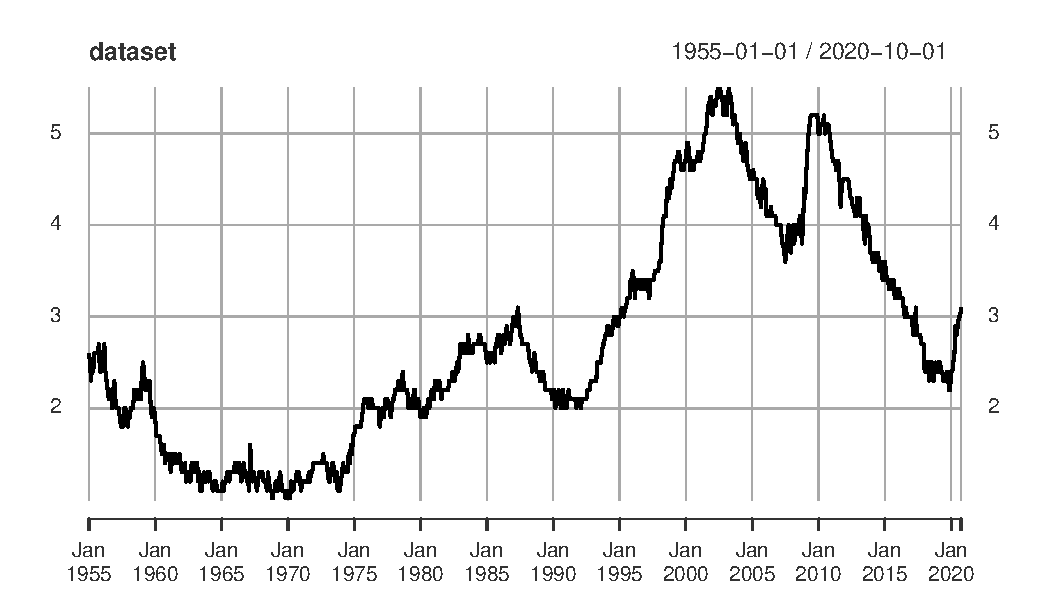
\includegraphics[width=\maxwidth]{figure/unnamed-chunk-18-1} 

\end{knitrout}
        \end{figure}


\section{Outliers}

    Antes de estimar os modelos, detectamos e removemos outliers. No teste abaixo, cinco tipos de outliers são considerados: outliers aditivos, mudanças de nível, mudanças temporárias, outliers inovadores e mudanças de nível sazonal. O teste segue a metodolodia de \cite{chungliu}.

\begin{knitrout}
\definecolor{shadecolor}{rgb}{0.969, 0.969, 0.969}\color{fgcolor}\begin{kframe}
\begin{alltt}
\hlstd{ol} \hlkwb{<-} \hlkwd{tso}\hlstd{(}\hlkwd{ts}\hlstd{(dataset))}
\hlstd{ol}
\end{alltt}
\begin{verbatim}
## Series: ts(dataset) 
## Regression with ARIMA(0,1,1) errors 
## 
## Coefficients:
##           ma1   AO147
##       -0.1885  0.3986
## s.e.   0.0365  0.0792
## 
## sigma^2 estimated as 0.01059:  log likelihood=675.7
## AIC=-1345.4   AICc=-1345.37   BIC=-1331.39
## 
## Outliers:
##   type ind time coefhat tstat
## 1   AO 147  147  0.3986 5.032
\end{verbatim}
\end{kframe}
\end{knitrout}
  
    Considerando o resultado do teste do \textit{chunk} anterior, substituimos o valor outlier com a função \textit{tsclean}.

\begin{knitrout}
\definecolor{shadecolor}{rgb}{0.969, 0.969, 0.969}\color{fgcolor}\begin{kframe}
\begin{alltt}
\hlstd{dataset} \hlkwb{<-} \hlkwd{tsclean}\hlstd{(dataset)}
\end{alltt}
\end{kframe}
\end{knitrout}
  
    No próximo \textit{chunk} apresentamos o sumário dos novos dados, junto ao gráfico dos novos dados.
  
\begin{knitrout}
\definecolor{shadecolor}{rgb}{0.969, 0.969, 0.969}\color{fgcolor}\begin{kframe}
\begin{alltt}
\hlkwd{summary}\hlstd{(dataset)}
\end{alltt}
\begin{verbatim}
##      Index                         Value     
##  Min.   :1955-01-01 00:00:00   Min.   :1.00  
##  1st Qu.:1971-06-08 12:00:00   1st Qu.:1.90  
##  Median :1987-11-16 00:00:00   Median :2.45  
##  Mean   :1987-11-16 00:25:31   Mean   :2.74  
##  3rd Qu.:2004-04-23 12:00:00   3rd Qu.:3.60  
##  Max.   :2020-10-01 00:00:00   Max.   :5.50
\end{verbatim}
\end{kframe}
\end{knitrout}

    \begin{figure}[H]
    \caption{Série Temporal sem Outliers}
    \centering
\begin{knitrout}
\definecolor{shadecolor}{rgb}{0.969, 0.969, 0.969}\color{fgcolor}\begin{kframe}
\begin{alltt}
\hlkwd{plot}\hlstd{(dataset)}
\end{alltt}
\end{kframe}
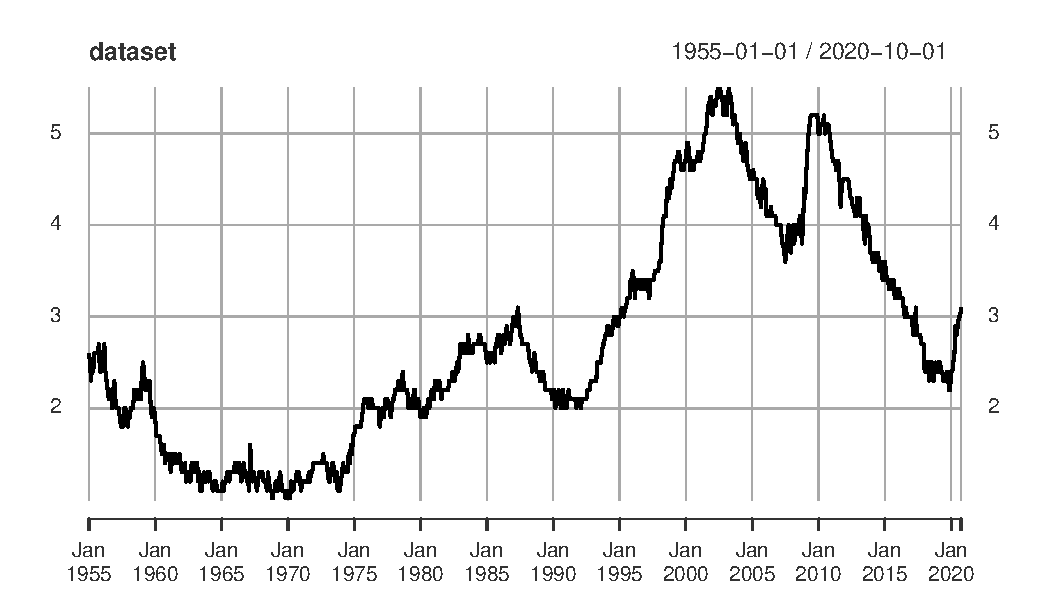
\includegraphics[width=\maxwidth]{figure/unnamed-chunk-22-1} 

\end{knitrout}
    \end{figure}


\section{Quebras Estruturais}

    Nesta seção testamos a existência de quebra estrutural na série. No caso de existência de quebra estrutural, estimamos a data de quebra.

    \subsection{Processo de Flutuação Empírica}
    
        Priemeiramente, calculamos o processo de flutuação empírica e o apresentamos no gráfico abaixo.
    
\begin{knitrout}
\definecolor{shadecolor}{rgb}{0.969, 0.969, 0.969}\color{fgcolor}\begin{kframe}
\begin{alltt}
\hlstd{efp1} \hlkwb{<-} \hlkwd{efp}\hlstd{(dataset}\hlopt{~}\hlnum{1}\hlstd{,} \hlkwc{type}\hlstd{=}\hlstr{"OLS-CUSUM"}\hlstd{)}
\end{alltt}
\end{kframe}
\end{knitrout}

        \begin{figure}[H]
        \caption{Processo de Flutuação Empírica}
        \centering
\begin{knitrout}
\definecolor{shadecolor}{rgb}{0.969, 0.969, 0.969}\color{fgcolor}\begin{kframe}
\begin{alltt}
\hlkwd{plot}\hlstd{(efp1)}
\end{alltt}
\end{kframe}
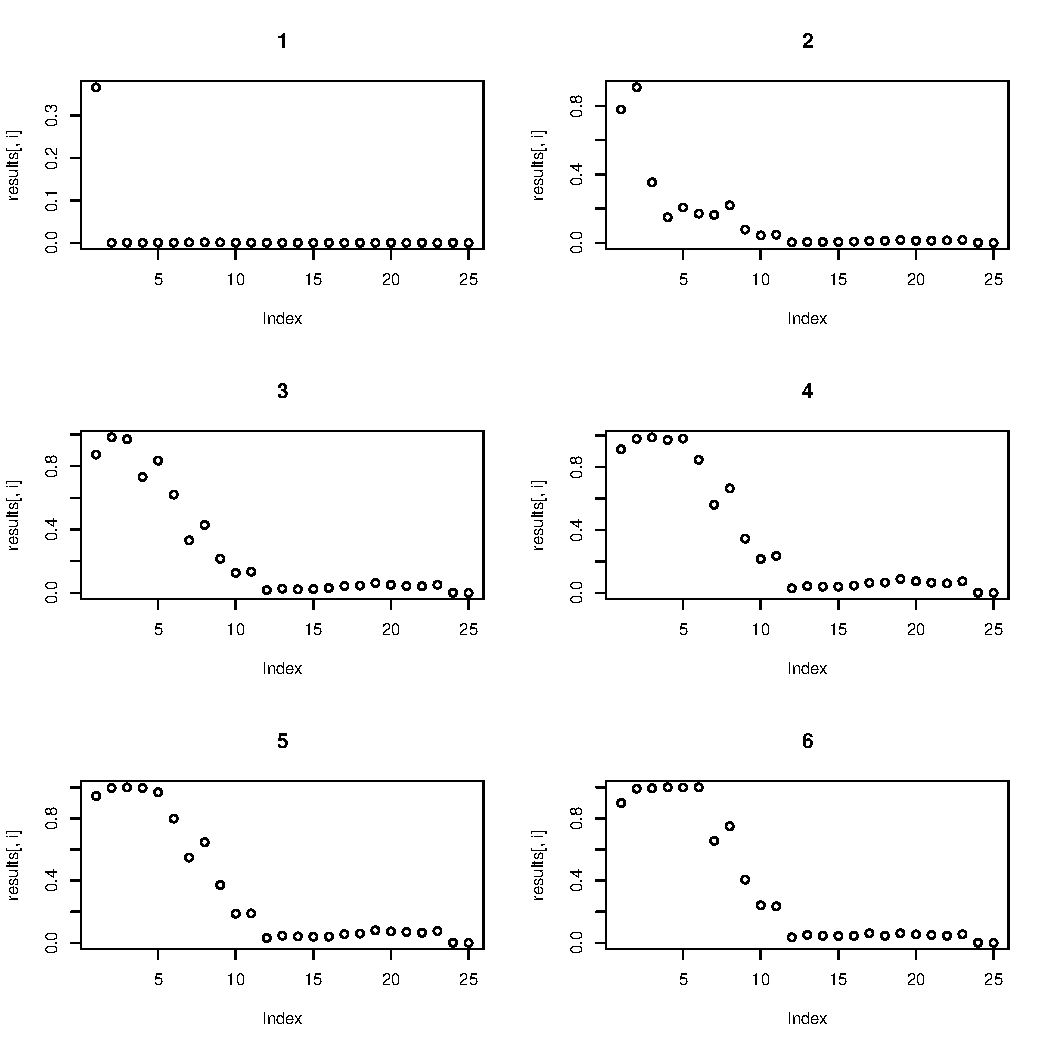
\includegraphics[width=\maxwidth]{figure/unnamed-chunk-24-1} 

\end{knitrout}
        \end{figure}
        
        O gráfico mostra que o processo ultrapassa os pontos críticos do intervalo de confiança, indicando que existe quebra estrutural na série temporal.

    \subsection{Teste de Existência de Quebra Estrutural}
    
        Na subseção anterior verificamos que o processo de flutuação empírica ultrapassa os limites do intervalo de confiança. Agora, testamos a hipótese de quebra estrutural.
    
\begin{knitrout}
\definecolor{shadecolor}{rgb}{0.969, 0.969, 0.969}\color{fgcolor}\begin{kframe}
\begin{alltt}
\hlkwd{sctest}\hlstd{(dataset}\hlopt{~}\hlnum{1}\hlstd{,} \hlkwc{type}\hlstd{=}\hlstr{"OLS-CUSUM"}\hlstd{)}
\end{alltt}
\begin{verbatim}
## 
## 	OLS-based CUSUM test
## 
## data:  dataset ~ 1
## S0 = 11.284, p-value < 2.2e-16
\end{verbatim}
\end{kframe}
\end{knitrout}

        O teste rejeita a hipótese nula de não existência de quebra estrutural, portanto podemos considerar que existe quebra estrutural na série temporal.
    
    \subsection{Estimação da Data da Quebra Estrutural}
    
        A estimativa de data mais provavél de quebra estrutural é o ponto do processo de flutuação empírica que mais se distancia dos pontos máximos do intervalo de confiança. Então, verificamos qual é esse valor.
    
\begin{knitrout}
\definecolor{shadecolor}{rgb}{0.969, 0.969, 0.969}\color{fgcolor}\begin{kframe}
\begin{alltt}
\hlstd{point} \hlkwb{<-} \hlkwd{which.min}\hlstd{(efp1}\hlopt{$}\hlstd{process)}
\hlstd{point}
\end{alltt}
\begin{verbatim}
## [1] 468
\end{verbatim}
\end{kframe}
\end{knitrout}

    \subsection{Divisão da Série Temporal}
    
        Na subseção anterior estimamos o ponto mais provável de quebra estrutural. Agora, separamos a série temporal original nesse ponto, como objetivo de obter uma série temporal para cada processo gerador.
    
\begin{knitrout}
\definecolor{shadecolor}{rgb}{0.969, 0.969, 0.969}\color{fgcolor}\begin{kframe}
\begin{alltt}
\hlstd{data1} \hlkwb{<-} \hlstd{dataset[}\hlnum{1}\hlopt{:}\hlstd{point}\hlopt{-}\hlnum{1}\hlstd{]}
\hlstd{data2} \hlkwb{<-} \hlstd{dataset[point}\hlopt{:}\hlkwd{length}\hlstd{(dataset)]}
\end{alltt}
\end{kframe}
\end{knitrout}
    
        Abaixo apresentamos os sumários das duas novas séries temporais.

\begin{knitrout}
\definecolor{shadecolor}{rgb}{0.969, 0.969, 0.969}\color{fgcolor}\begin{kframe}
\begin{alltt}
\hlkwd{summary}\hlstd{(data1)}
\end{alltt}
\begin{verbatim}
##      Index                         Value      
##  Min.   :1955-01-01 00:00:00   Min.   :1.000  
##  1st Qu.:1964-09-16 00:00:00   1st Qu.:1.300  
##  Median :1974-06-01 00:00:00   Median :2.000  
##  Mean   :1974-06-01 08:47:16   Mean   :1.905  
##  3rd Qu.:1984-02-15 12:00:00   3rd Qu.:2.300  
##  Max.   :1993-11-01 00:00:00   Max.   :3.100
\end{verbatim}
\begin{alltt}
\hlkwd{summary}\hlstd{(data2)}
\end{alltt}
\begin{verbatim}
##      Index                         Value      
##  Min.   :1993-12-01 00:00:00   Min.   :2.200  
##  1st Qu.:2000-08-16 12:00:00   1st Qu.:3.200  
##  Median :2007-05-01 00:00:00   Median :4.000  
##  Mean   :2007-05-02 04:00:44   Mean   :3.948  
##  3rd Qu.:2014-01-16 12:00:00   3rd Qu.:4.700  
##  Max.   :2020-10-01 00:00:00   Max.   :5.500
\end{verbatim}
\end{kframe}
\end{knitrout}



\section{Primeira Parte da Série Temporal}

    \subsection{Definição da Ordem de Integração}
    
        O primeiro passo na metodologia Box-Jenkins (\cite{boxjenkins}) é a definição da ordem de integração da série temporal .
    
        \subsubsection{Análise da Série Original}
        
            Começamos o processo de definição da ordem de integração analisando o gráfico da série temporal.
        
            \begin{figure}[H]
            \caption{Série Temporal}
            \centering
\begin{knitrout}
\definecolor{shadecolor}{rgb}{0.969, 0.969, 0.969}\color{fgcolor}\begin{kframe}
\begin{alltt}
\hlkwd{plot}\hlstd{(data1)}
\end{alltt}
\end{kframe}
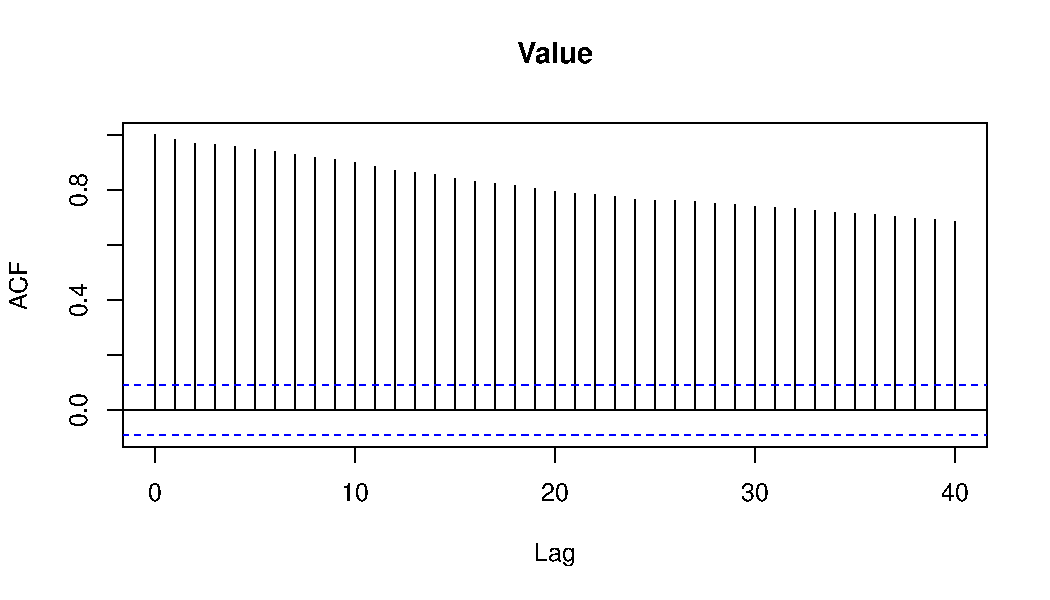
\includegraphics[width=\maxwidth]{figure/unnamed-chunk-29-1} 

\end{knitrout}
            \end{figure}
            
            O gráfico assemelha-se a um passeio aleatório, portanto, indicandio a presença de raíz unitária. Para coletar mais indícios analisamos abaixo a função de autocorrelação e a função de autocorrelação parcial.
            
            \begin{figure}[H]
            \caption{FAC da Série Temporal}
            \centering
\begin{knitrout}
\definecolor{shadecolor}{rgb}{0.969, 0.969, 0.969}\color{fgcolor}\begin{kframe}
\begin{alltt}
\hlkwd{acf}\hlstd{(}\hlkwd{as.matrix}\hlstd{(data1),} \hlkwc{lag.max}\hlstd{=}\hlnum{60}\hlstd{)}
\end{alltt}
\end{kframe}
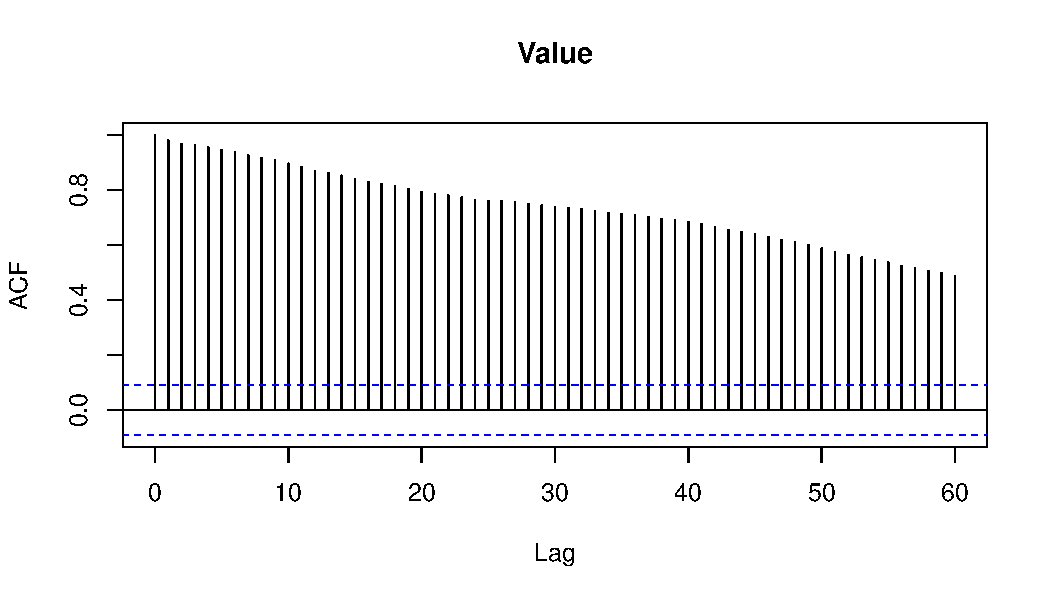
\includegraphics[width=\maxwidth]{figure/unnamed-chunk-30-1} 

\end{knitrout}
            \end{figure}
            
            \begin{figure}[H]
            \caption{FACP da Série Temporal}
            \centering
\begin{knitrout}
\definecolor{shadecolor}{rgb}{0.969, 0.969, 0.969}\color{fgcolor}\begin{kframe}
\begin{alltt}
\hlkwd{pacf}\hlstd{(}\hlkwd{as.matrix}\hlstd{(data1),} \hlkwc{lag.max}\hlstd{=}\hlnum{60}\hlstd{)}
\end{alltt}
\end{kframe}
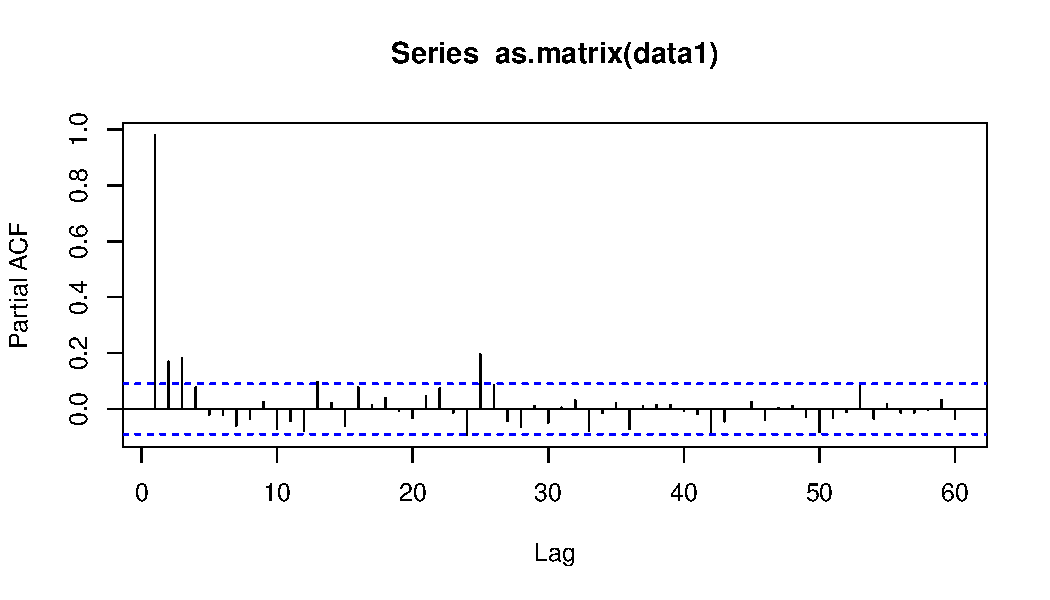
\includegraphics[width=\maxwidth]{figure/unnamed-chunk-31-1} 

\end{knitrout}
            \end{figure}
            
            A função de autocorrelação aparentemente possui decaimento lento, indicando possibilidade de raiz unitária. Para testar a hipótese de presença de raiz unitária cutilizamos o teste Dickey-Fuller aumentado (\cite{adf}). O teste será realizado sem \textit{drift} ou tendência, pois a visualização do gráfico da série temporal indica a não presença de tais. Para escolher o lag do teste, começaremos pelo lag 1 e, caso os resíduos do teste forem ruído branco, aceitamos o lag. Caso os resíduos não apresentarem comportamento de ruído branco, repetimos os passos com o lag imediatamente maior. No \textit{chunk} abaixo realizamos esse passos para encontrar o menor lag que retorna resíduos que sejam ruído branco.


\begin{knitrout}
\definecolor{shadecolor}{rgb}{0.969, 0.969, 0.969}\color{fgcolor}\begin{kframe}
\begin{alltt}
\hlstd{lag} \hlkwb{<-} \hlkwd{select_adf}\hlstd{(data1}\hlopt{$}\hlstd{Value,}\hlstr{"none"}\hlstd{)}
\hlstd{lag}
\end{alltt}
\begin{verbatim}
## [1] 24
\end{verbatim}
\end{kframe}
\end{knitrout}

            Os resultados dos passos anteriores indicam que o menor lag para o teste é o 24, então realizamos o teste com essa ordem.
            
\begin{knitrout}
\definecolor{shadecolor}{rgb}{0.969, 0.969, 0.969}\color{fgcolor}\begin{kframe}
\begin{alltt}
\hlstd{adf} \hlkwb{<-} \hlkwd{ur.df}\hlstd{(data1}\hlopt{$}\hlstd{Value,} \hlkwc{type}\hlstd{=}\hlstr{"none"}\hlstd{,} \hlkwc{lags}\hlstd{=lag)}
\end{alltt}
\end{kframe}
\end{knitrout}

            Abaixo analisamos os resíduos do teste.
            
            \begin{figure}[H]
            \caption{Resíduos}
            \centering
\begin{knitrout}
\definecolor{shadecolor}{rgb}{0.969, 0.969, 0.969}\color{fgcolor}\begin{kframe}
\begin{alltt}
\hlkwd{par}\hlstd{(}\hlkwc{mfrow} \hlstd{=} \hlkwd{c}\hlstd{(}\hlnum{2}\hlstd{,}\hlnum{2}\hlstd{))}
\hlkwd{plot}\hlstd{(adf}\hlopt{@}\hlkwc{res}\hlstd{,} \hlkwc{type}\hlstd{=}\hlstr{'l'}\hlstd{,} \hlkwc{main}\hlstd{=}\hlstr{'Residuals'}\hlstd{)}
\hlkwd{plot}\hlstd{(}\hlkwd{all_box}\hlstd{(adf}\hlopt{@}\hlkwc{res}\hlstd{),} \hlkwc{main}\hlstd{=}\hlstr{'Ljung-Box'}\hlstd{)}
\hlkwd{acf}\hlstd{(}\hlkwd{as.matrix}\hlstd{(adf}\hlopt{@}\hlkwc{res}\hlstd{),} \hlkwc{lag.max}\hlstd{=}\hlnum{60}\hlstd{)}
\hlkwd{pacf}\hlstd{(}\hlkwd{as.matrix}\hlstd{(adf}\hlopt{@}\hlkwc{res}\hlstd{),} \hlkwc{lag.max}\hlstd{=}\hlnum{60}\hlstd{)}
\end{alltt}
\end{kframe}
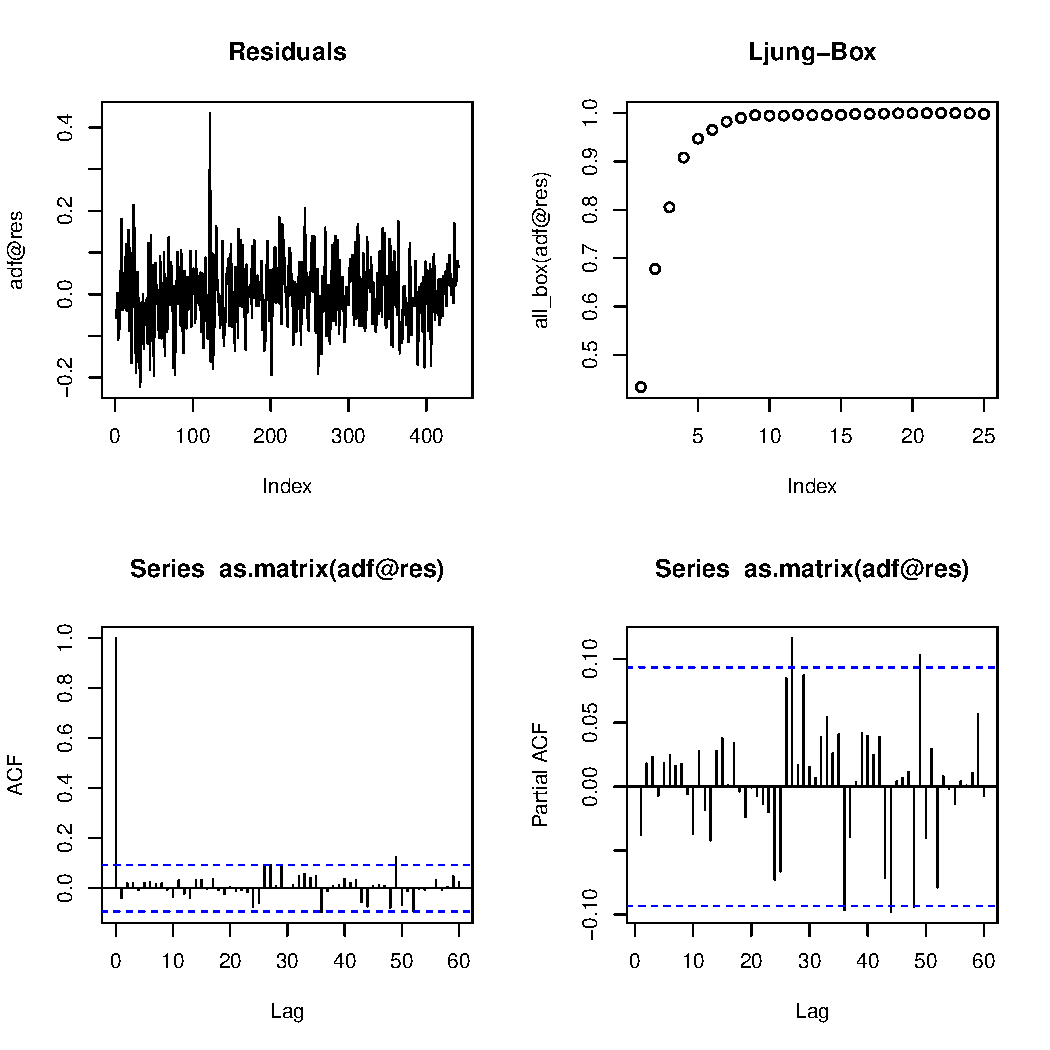
\includegraphics[width=\maxwidth]{figure/unnamed-chunk-34-1} 

\end{knitrout}
            \end{figure}

            Tanto o gráfico dos resíduos quanto os gráficos das funções de autocorrelação e autocorrelação parcial indicam que os resíduos do teste se comportam como ruído branco. Os p-valores do teste de Ljung-Box não rejeitam a hipótese de independência dos resíduos.

            Agora, visualizamos as estatísticas do teste e os valores críticos        
            
\begin{knitrout}
\definecolor{shadecolor}{rgb}{0.969, 0.969, 0.969}\color{fgcolor}\begin{kframe}
\begin{alltt}
\hlstd{adf}\hlopt{@}\hlkwc{teststat}
\end{alltt}
\begin{verbatim}
##                tau1
## statistic 0.1471326
\end{verbatim}
\begin{alltt}
\hlstd{adf}\hlopt{@}\hlkwc{cval}
\end{alltt}
\begin{verbatim}
##       1pct  5pct 10pct
## tau1 -2.58 -1.95 -1.62
\end{verbatim}
\end{kframe}
\end{knitrout}

            O valor da estatística do teste é de 0,1471. Os valores críticos para o teste são de -2,58 (1\%), -1,95 (5\%) e -1,62 (10\%). Sendo assim, o valor do teste não ultrapassou os valores críticos para nenhum grau de significância. O teste indica que não há evidências suficientes para rejeitarmos a hipótese nula de presença de raíz unitária.

        \subsubsection{Diferenciação}
        
            Como tentativa para estacionarizar a série, aplicamos a primeira diferença.

\begin{knitrout}
\definecolor{shadecolor}{rgb}{0.969, 0.969, 0.969}\color{fgcolor}\begin{kframe}
\begin{alltt}
\hlstd{data1}\hlopt{$}\hlstd{Diff} \hlkwb{<-} \hlkwd{diff}\hlstd{(data1)}
\end{alltt}
\end{kframe}
\end{knitrout}

            Abaixo, o sumário dos novos dados.
            
\begin{knitrout}
\definecolor{shadecolor}{rgb}{0.969, 0.969, 0.969}\color{fgcolor}\begin{kframe}
\begin{alltt}
\hlkwd{summary}\hlstd{(data1)}
\end{alltt}
\begin{verbatim}
##      Index                         Value            Diff           
##  Min.   :1955-01-01 00:00:00   Min.   :1.000   Min.   :-0.3000000  
##  1st Qu.:1964-09-16 00:00:00   1st Qu.:1.300   1st Qu.:-0.1000000  
##  Median :1974-06-01 00:00:00   Median :2.000   Median : 0.0000000  
##  Mean   :1974-06-01 08:47:16   Mean   :1.905   Mean   : 0.0002146  
##  3rd Qu.:1984-02-15 12:00:00   3rd Qu.:2.300   3rd Qu.: 0.1000000  
##  Max.   :1993-11-01 00:00:00   Max.   :3.100   Max.   : 0.5000000  
##                                                NA's   :1
\end{verbatim}
\end{kframe}
\end{knitrout}
      
        \subsubsection{Análise da Primeira Diferença}
        
            Começamos a nova análise analisando o gráfico da primeira diferença da série temporal.
        
            \begin{figure}[H]
            \caption{Primeira Diferença}
            \centering
\begin{knitrout}
\definecolor{shadecolor}{rgb}{0.969, 0.969, 0.969}\color{fgcolor}\begin{kframe}
\begin{alltt}
\hlkwd{plot}\hlstd{(data1}\hlopt{$}\hlstd{Diff)}
\end{alltt}
\end{kframe}
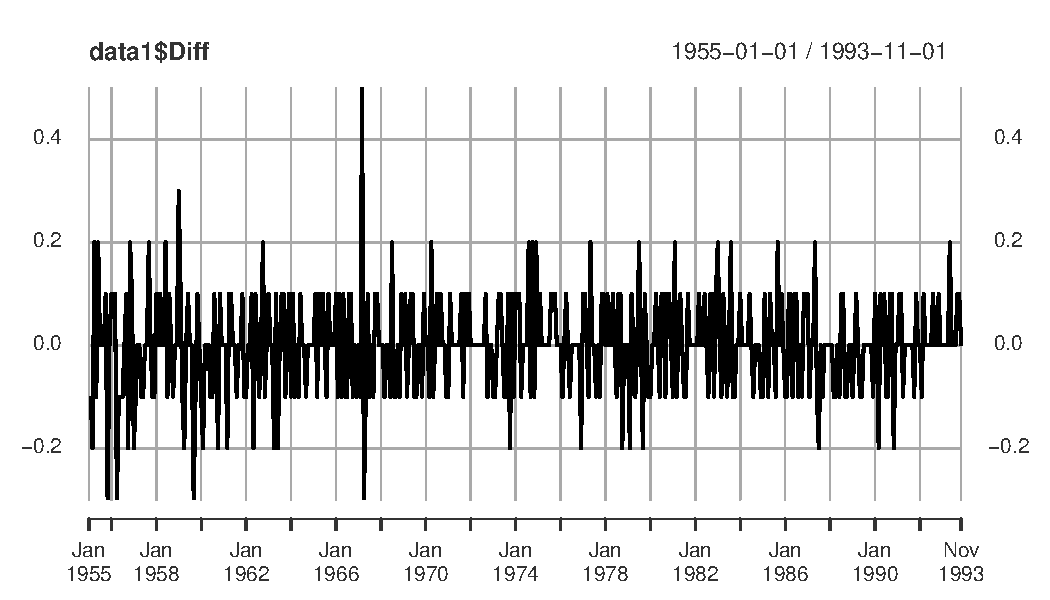
\includegraphics[width=\maxwidth]{figure/unnamed-chunk-38-1} 

\end{knitrout}
            \end{figure}
            
            A analise visual do gráfico sugere variação em torno de uma média sem distanciamento grande por longos períodos, portanto, indica que a estacionariedade da série foi obtida na primeira diferenciação.
            
            \begin{figure}[H]
            \caption{FAC da Primeira Diferença}
            \centering
\begin{knitrout}
\definecolor{shadecolor}{rgb}{0.969, 0.969, 0.969}\color{fgcolor}\begin{kframe}
\begin{alltt}
\hlkwd{acf}\hlstd{(}\hlkwd{as.matrix}\hlstd{(}\hlkwd{na.omit}\hlstd{(data1}\hlopt{$}\hlstd{Diff)),} \hlkwc{lag.max}\hlstd{=}\hlnum{60}\hlstd{)}
\end{alltt}
\end{kframe}
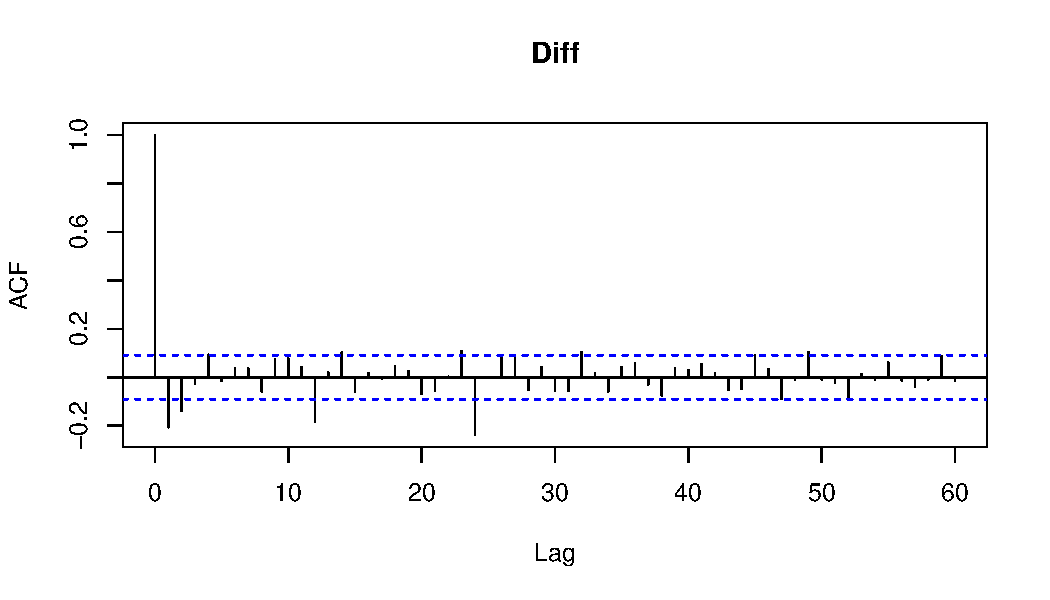
\includegraphics[width=\maxwidth]{figure/unnamed-chunk-39-1} 

\end{knitrout}
            \end{figure}
            
            \begin{figure}[H]
            \caption{FACP da Primeira Diferença}
            \centering
\begin{knitrout}
\definecolor{shadecolor}{rgb}{0.969, 0.969, 0.969}\color{fgcolor}\begin{kframe}
\begin{alltt}
\hlkwd{pacf}\hlstd{(}\hlkwd{as.matrix}\hlstd{(}\hlkwd{na.omit}\hlstd{(data1}\hlopt{$}\hlstd{Diff)),} \hlkwc{lag.max}\hlstd{=}\hlnum{60}\hlstd{)}
\end{alltt}
\end{kframe}
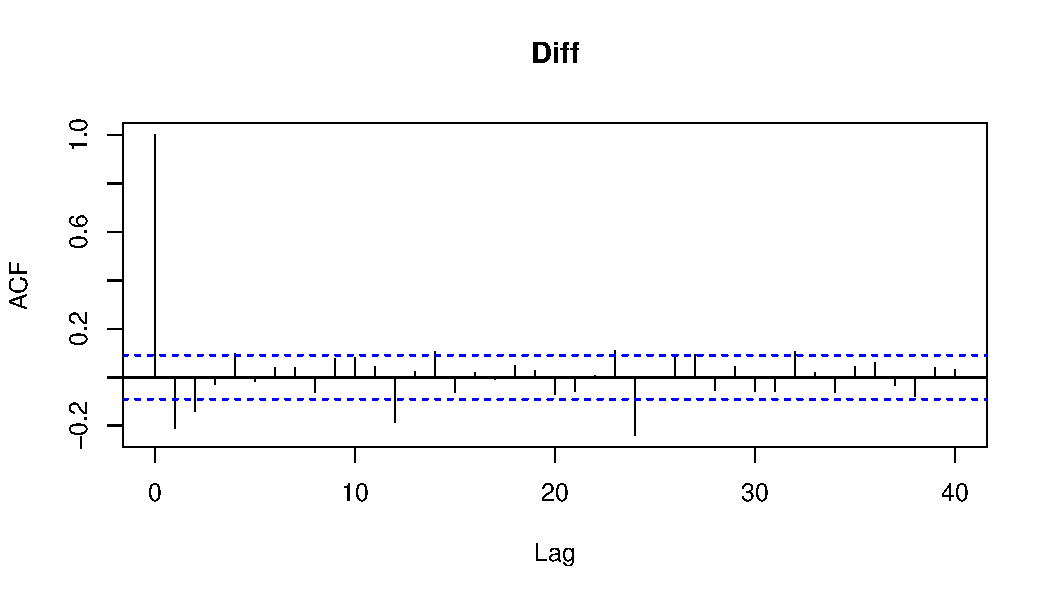
\includegraphics[width=\maxwidth]{figure/unnamed-chunk-40-1} 

\end{knitrout}
            \end{figure}
            
            A análise dos gráficos pós diferenciação indica rápido decaimento nas funções ACF e PACF, reforçando a hipótese de que não há raíz unitária. Agora testaremos, com o teste de Dickey-Fuller aumentado, a presença de raiz unitária. Não adicionaremos drift ou tendância no teste pois não há indício pelo gráfico da série de existência de algum desses parâmetros. Seguiremos os passos descritos acima, quando aplicamos o teste na série temporal original.

\begin{knitrout}
\definecolor{shadecolor}{rgb}{0.969, 0.969, 0.969}\color{fgcolor}\begin{kframe}
\begin{alltt}
\hlstd{lag} \hlkwb{<-} \hlkwd{select_adf}\hlstd{(}\hlkwd{na.omit}\hlstd{(data1}\hlopt{$}\hlstd{Diff),}\hlstr{"none"}\hlstd{)}
\hlstd{lag}
\end{alltt}
\begin{verbatim}
## [1] 23
\end{verbatim}
\end{kframe}
\end{knitrout}

          Os resultados dos passos anteriores indicam que o menor lag para o teste é o 23, então realizamos o teste com essa ordem.
            
\begin{knitrout}
\definecolor{shadecolor}{rgb}{0.969, 0.969, 0.969}\color{fgcolor}\begin{kframe}
\begin{alltt}
\hlstd{adf} \hlkwb{<-} \hlkwd{ur.df}\hlstd{(}\hlkwd{na.omit}\hlstd{(data1}\hlopt{$}\hlstd{Diff),}\hlstr{"none"}\hlstd{,}\hlkwc{lags}\hlstd{=lag)}
\end{alltt}
\end{kframe}
\end{knitrout}

            \begin{figure}[H]
            \caption{Resíduos}
            \centering
\begin{knitrout}
\definecolor{shadecolor}{rgb}{0.969, 0.969, 0.969}\color{fgcolor}\begin{kframe}
\begin{alltt}
\hlkwd{par}\hlstd{(}\hlkwc{mfrow} \hlstd{=} \hlkwd{c}\hlstd{(}\hlnum{2}\hlstd{,}\hlnum{2}\hlstd{))}
\hlkwd{plot}\hlstd{(adf}\hlopt{@}\hlkwc{res}\hlstd{,} \hlkwc{type}\hlstd{=}\hlstr{'l'}\hlstd{,} \hlkwc{main}\hlstd{=}\hlstr{'Residuals'}\hlstd{)}
\hlkwd{plot}\hlstd{(}\hlkwd{all_box}\hlstd{(adf}\hlopt{@}\hlkwc{res}\hlstd{),} \hlkwc{main}\hlstd{=}\hlstr{'Ljung-Box'}\hlstd{)}
\hlkwd{acf}\hlstd{(}\hlkwd{as.matrix}\hlstd{(adf}\hlopt{@}\hlkwc{res}\hlstd{),} \hlkwc{lag.max}\hlstd{=}\hlnum{60}\hlstd{)}
\hlkwd{pacf}\hlstd{(}\hlkwd{as.matrix}\hlstd{(adf}\hlopt{@}\hlkwc{res}\hlstd{),} \hlkwc{lag.max}\hlstd{=}\hlnum{60}\hlstd{)}
\end{alltt}
\end{kframe}
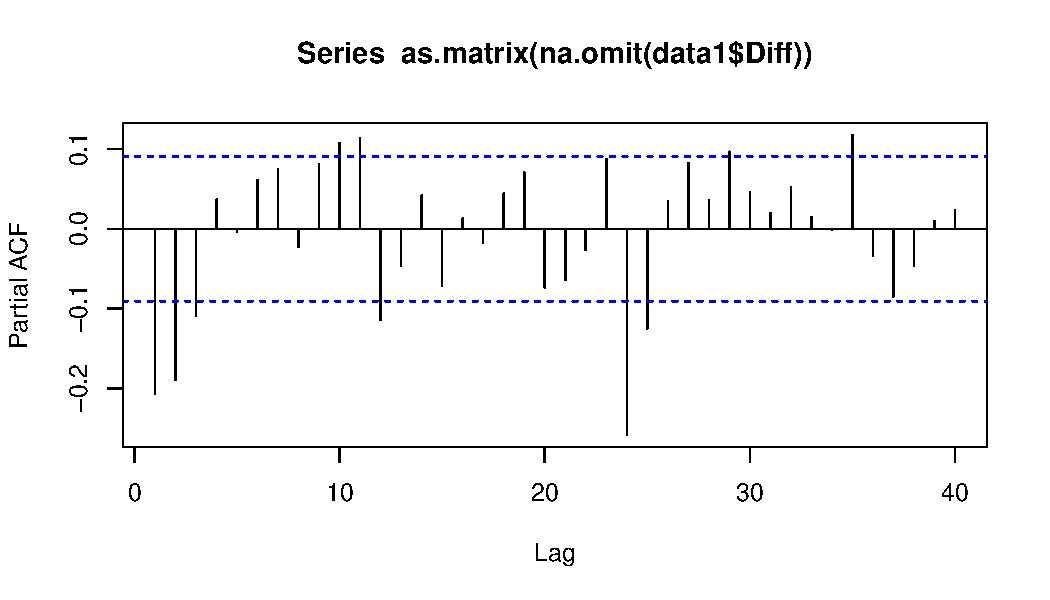
\includegraphics[width=\maxwidth]{figure/unnamed-chunk-43-1} 

\end{knitrout}
            \end{figure}

            Tanto o gráfico dos resíduos quanto os gráficos das funções de autocorrelação e autocorrelação parcial indicam que os resíduos do teste se comportam como ruído branco. Os p-valores do teste de Ljung-Box não rejeitam a hipótese de independência dos resíduos.

            Agora, visualizamos as estatísticas do teste e os valores críticos        
            
\begin{knitrout}
\definecolor{shadecolor}{rgb}{0.969, 0.969, 0.969}\color{fgcolor}\begin{kframe}
\begin{alltt}
\hlstd{adf}\hlopt{@}\hlkwc{teststat}
\end{alltt}
\begin{verbatim}
##              tau1
## statistic -5.1105
\end{verbatim}
\begin{alltt}
\hlstd{adf}\hlopt{@}\hlkwc{cval}
\end{alltt}
\begin{verbatim}
##       1pct  5pct 10pct
## tau1 -2.58 -1.95 -1.62
\end{verbatim}
\end{kframe}
\end{knitrout}
            
            O valor da estatística do teste é de -5,1105. Os valores críticos para o teste são de -2,58 (1\%), -1,95 (5\%) e -1,62 (10\%). Sendo assim, o valor do teste ultrapassou os valores críticos para todos os graus de significância. O teste aponta que não há evidências suficientes de presença de raíz unitária. Portanto, consideramos a série estacionária após a primeira diferenciação. O resultado obtido é, então, que a série temporal original é integrada de ordem 1 - I(1).
            
        \subsubsection{Diferença Sazonal}
    
            A função de autocorrelação indica que existem lags sazonais significativos, no entando, o decaimento é rápido, indicanco não existência de raiz unitária sazonal.Testamos a seguir a hipótese nula de não presença de raiz unitária sazonal com o teste de Canova e Hansen (\cite{ch}).
          
\begin{knitrout}
\definecolor{shadecolor}{rgb}{0.969, 0.969, 0.969}\color{fgcolor}\begin{kframe}
\begin{alltt}
\hlstd{ch} \hlkwb{=} \hlkwd{ch.test}\hlstd{(}\hlkwd{ts}\hlstd{(}\hlkwd{na.omit}\hlstd{(data1}\hlopt{$}\hlstd{Diff),} \hlkwc{frequency}\hlstd{=}\hlnum{12}\hlstd{),} \hlkwc{type}\hlstd{=}\hlstr{"dummy"}\hlstd{,} \hlkwc{sid}\hlstd{=}\hlkwd{c}\hlstd{(}\hlnum{1}\hlopt{:}\hlnum{12}\hlstd{))}
\hlstd{ch}\hlopt{$}\hlstd{pvalues}
\end{alltt}
\begin{verbatim}
## [1] 0.5464967
\end{verbatim}
\end{kframe}
\end{knitrout}

            O teste retornou um p-valor de 0.5465, o que significa que não podemos rejeitar a hipótese nula de não presença de raiz unitária sazonal.


    \subsection{Identificação das Possíveis Formas Funcionais}
    
        \begin{figure}[H]
        \caption{FAC da Primeira Diferença}
        \centering
\begin{knitrout}
\definecolor{shadecolor}{rgb}{0.969, 0.969, 0.969}\color{fgcolor}\begin{kframe}
\begin{alltt}
\hlkwd{acf}\hlstd{(}\hlkwd{as.matrix}\hlstd{(}\hlkwd{na.omit}\hlstd{(data1}\hlopt{$}\hlstd{Diff)),} \hlkwc{lag.max}\hlstd{=}\hlnum{60}\hlstd{)}
\end{alltt}
\end{kframe}
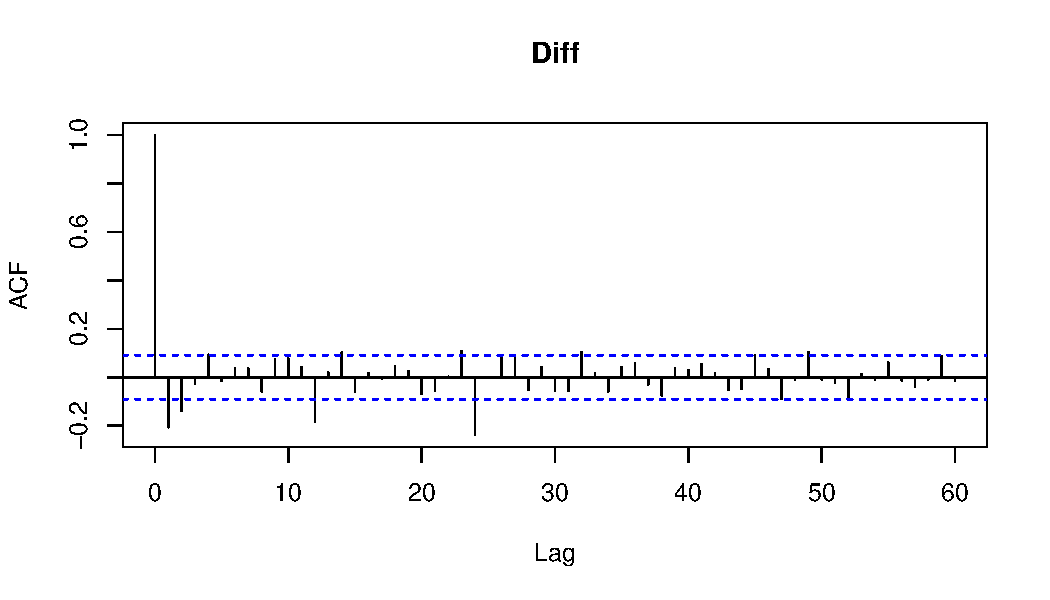
\includegraphics[width=\maxwidth]{figure/unnamed-chunk-46-1} 

\end{knitrout}
        \end{figure}
        
        A função de autocorrelação trunca após o segundo lag. Como mencionado anteriormente, a FAC da série da primeira diferença mostra que há decaimento rápido do padrão de sazonalidade (múltiplo de 12) a partir do lag número 24.
        
        
        \begin{figure}[H]
        \caption{FACP da Primeira Diferença}
        \centering
\begin{knitrout}
\definecolor{shadecolor}{rgb}{0.969, 0.969, 0.969}\color{fgcolor}\begin{kframe}
\begin{alltt}
\hlkwd{pacf}\hlstd{(}\hlkwd{as.matrix}\hlstd{(}\hlkwd{na.omit}\hlstd{(data1}\hlopt{$}\hlstd{Diff)),} \hlkwc{lag.max}\hlstd{=}\hlnum{60}\hlstd{)}
\end{alltt}
\end{kframe}
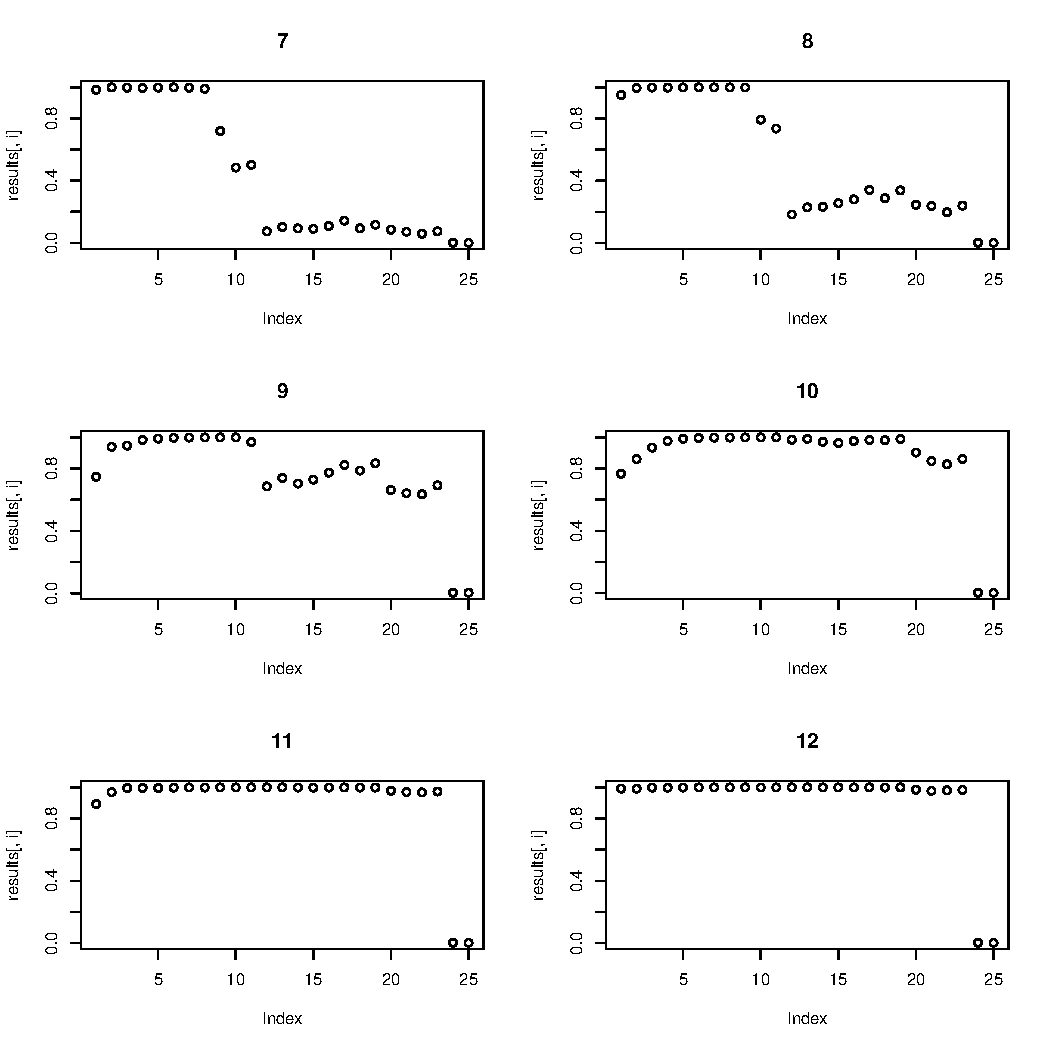
\includegraphics[width=\maxwidth]{figure/unnamed-chunk-47-1} 

\end{knitrout}
        \end{figure}

        A função de autocorrelação parcial tem até o terceiro lag significativo, enquanto mostra três lags significativos no fator sazonal.
        
        A análise das funções acima sugere que uma ordem máxima para o modelo SARIMA é (3,1,2)(3,0,2)12.


    \subsection{Estimação}
    
        Na subseção anterior definimos as ordems máximas do modelo SARIMA. Nesta seção vamos estimar todos os modelos até as ordens máximas, testar seus resíduos para checar se comportam-se como ruído branco e, finalmente, escolher os modelos que passam o teste dos resíduos que apresente melhores critério de informação (AIC e BIC). Esses passos são realizados no \textit{chunk} abaixo.

\begin{knitrout}
\definecolor{shadecolor}{rgb}{0.969, 0.969, 0.969}\color{fgcolor}\begin{kframe}
\begin{alltt}
\hlstd{order} \hlkwb{<-} \hlkwd{select_model}\hlstd{(data1}\hlopt{$}\hlstd{Value,}\hlnum{3}\hlstd{,}\hlnum{1}\hlstd{,}\hlnum{2}\hlstd{,}\hlnum{3}\hlstd{,}\hlnum{0}\hlstd{,}\hlnum{2}\hlstd{,}\hlnum{12}\hlstd{)}
\end{alltt}
\end{kframe}
\end{knitrout}
    
        Abaixo, as ordens dos melhores modelos pelos critérios AIC e BIC.

\begin{knitrout}
\definecolor{shadecolor}{rgb}{0.969, 0.969, 0.969}\color{fgcolor}\begin{kframe}
\begin{alltt}
\hlcom{# Ordem pelo critério AIC}
\hlkwd{print}\hlstd{(}\hlstr{"p q P Q"}\hlstd{)}
\end{alltt}
\begin{verbatim}
## [1] "p q P Q"
\end{verbatim}
\begin{alltt}
\hlstd{order[,}\hlnum{1}\hlstd{]}
\end{alltt}
\begin{verbatim}
## [1] 2 2 1 2
\end{verbatim}
\begin{alltt}
\hlcom{# Ordem pelo critério BIC}
\hlkwd{print}\hlstd{(}\hlstr{"p q P Q"}\hlstd{)}
\end{alltt}
\begin{verbatim}
## [1] "p q P Q"
\end{verbatim}
\begin{alltt}
\hlstd{order[,}\hlnum{2}\hlstd{]}
\end{alltt}
\begin{verbatim}
## [1] 2 2 0 2
\end{verbatim}
\end{kframe}
\end{knitrout}

        O modelo com melhor critério AIC é o SARIMA (2,1,2)(1,0,2)12, e o com melhor critério BIC é o SARIMA(2,1,2)(0,0,2)12. Pelo princípio da parcimônia, optamos pelo modelo mais simples (menos parâmetros), que apresenta menor critério BIC.
            
\begin{knitrout}
\definecolor{shadecolor}{rgb}{0.969, 0.969, 0.969}\color{fgcolor}\begin{kframe}
\begin{alltt}
\hlstd{model1} \hlkwb{<-} \hlkwd{sarima}\hlstd{(data1}\hlopt{$}\hlstd{Value,}
                 \hlnum{2}\hlstd{,} \hlnum{1}\hlstd{,} \hlnum{2}\hlstd{,}
                 \hlnum{0}\hlstd{,} \hlnum{0}\hlstd{,} \hlnum{2}\hlstd{,} \hlnum{12}\hlstd{)}
\end{alltt}
\end{kframe}
\end{knitrout}


    \subsection{Diagnóstico dos Resíduos}
    
        Nesta seção iremos fazer o diagnóstico dos resíduos. Para isso vamos analisar sua independência e homoscedasticidade.
        
        \subsubsection{Independência}
        
            Para analisar a independência dos resíduos analisamos o gráfico dos resíduos, a função de autocorrelação e a função de autocorrelação parcial.
        
            \begin{figure}[H]
            \caption{Resíduos}
            \centering
\begin{knitrout}
\definecolor{shadecolor}{rgb}{0.969, 0.969, 0.969}\color{fgcolor}\begin{kframe}
\begin{alltt}
\hlkwd{plot}\hlstd{(model1}\hlopt{$}\hlstd{fit}\hlopt{$}\hlstd{residuals)}
\end{alltt}
\end{kframe}
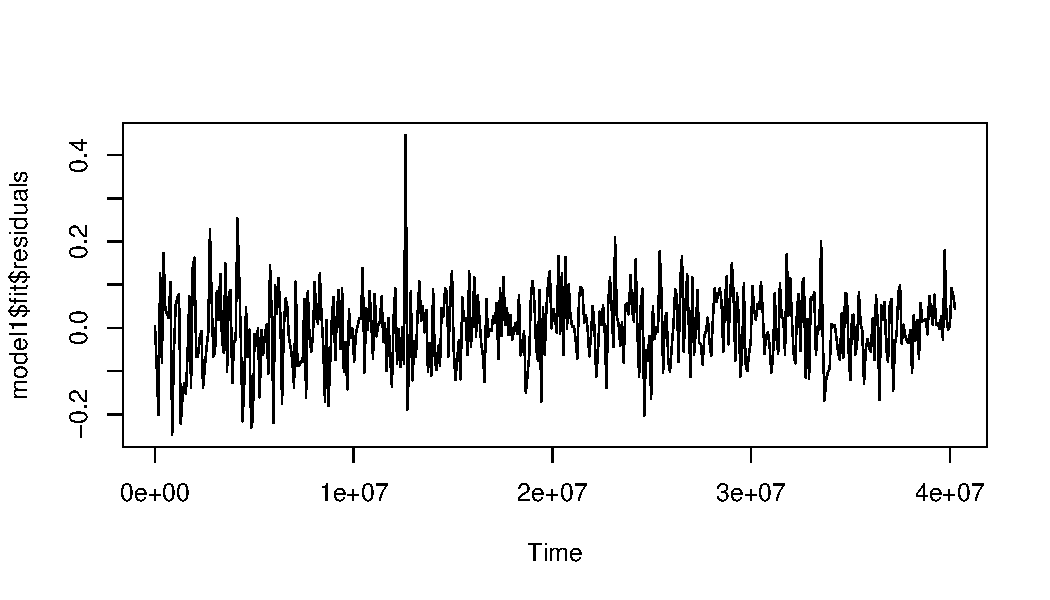
\includegraphics[width=\maxwidth]{figure/unnamed-chunk-49-1} 

\end{knitrout}
            \end{figure}
            
            \begin{figure}[H]
            \caption{FAC dos Resíduos}
            \centering          
\begin{knitrout}
\definecolor{shadecolor}{rgb}{0.969, 0.969, 0.969}\color{fgcolor}\begin{kframe}
\begin{alltt}
\hlkwd{acf}\hlstd{(}\hlkwd{as.matrix}\hlstd{(model1}\hlopt{$}\hlstd{fit}\hlopt{$}\hlstd{residuals),} \hlkwc{lag.max}\hlstd{=}\hlnum{40}\hlstd{)}
\end{alltt}
\end{kframe}
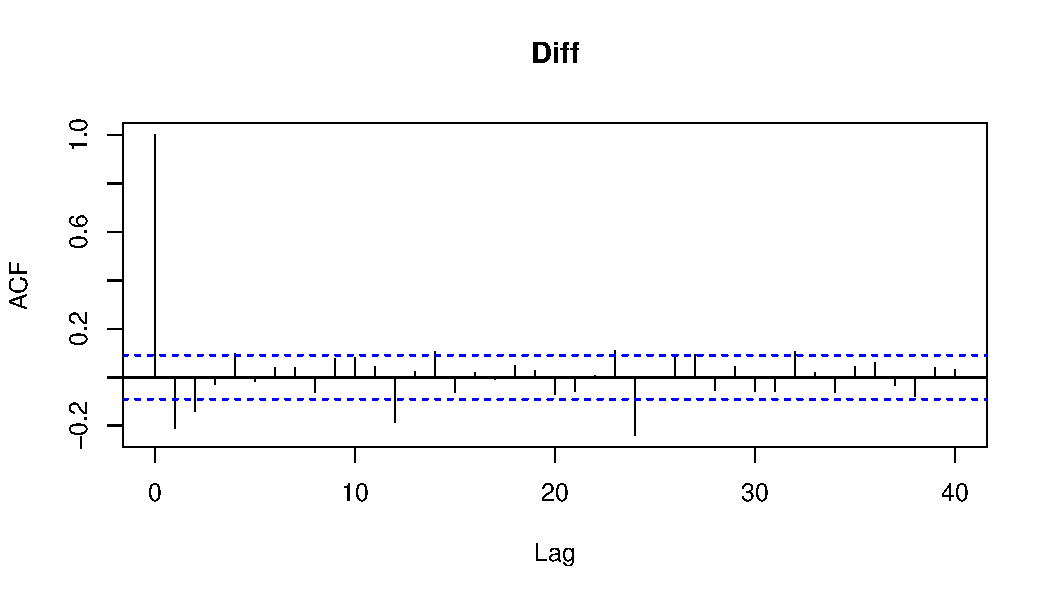
\includegraphics[width=\maxwidth]{figure/unnamed-chunk-50-1} 

\end{knitrout}
            \end{figure}
            
            \begin{figure}[H]
            \caption{FACP dos Resíduos}
            \centering          
\begin{knitrout}
\definecolor{shadecolor}{rgb}{0.969, 0.969, 0.969}\color{fgcolor}\begin{kframe}
\begin{alltt}
\hlkwd{pacf}\hlstd{(}\hlkwd{as.matrix}\hlstd{(model1}\hlopt{$}\hlstd{fit}\hlopt{$}\hlstd{residuals),} \hlkwc{lag.max}\hlstd{=}\hlnum{40}\hlstd{)}
\end{alltt}
\end{kframe}
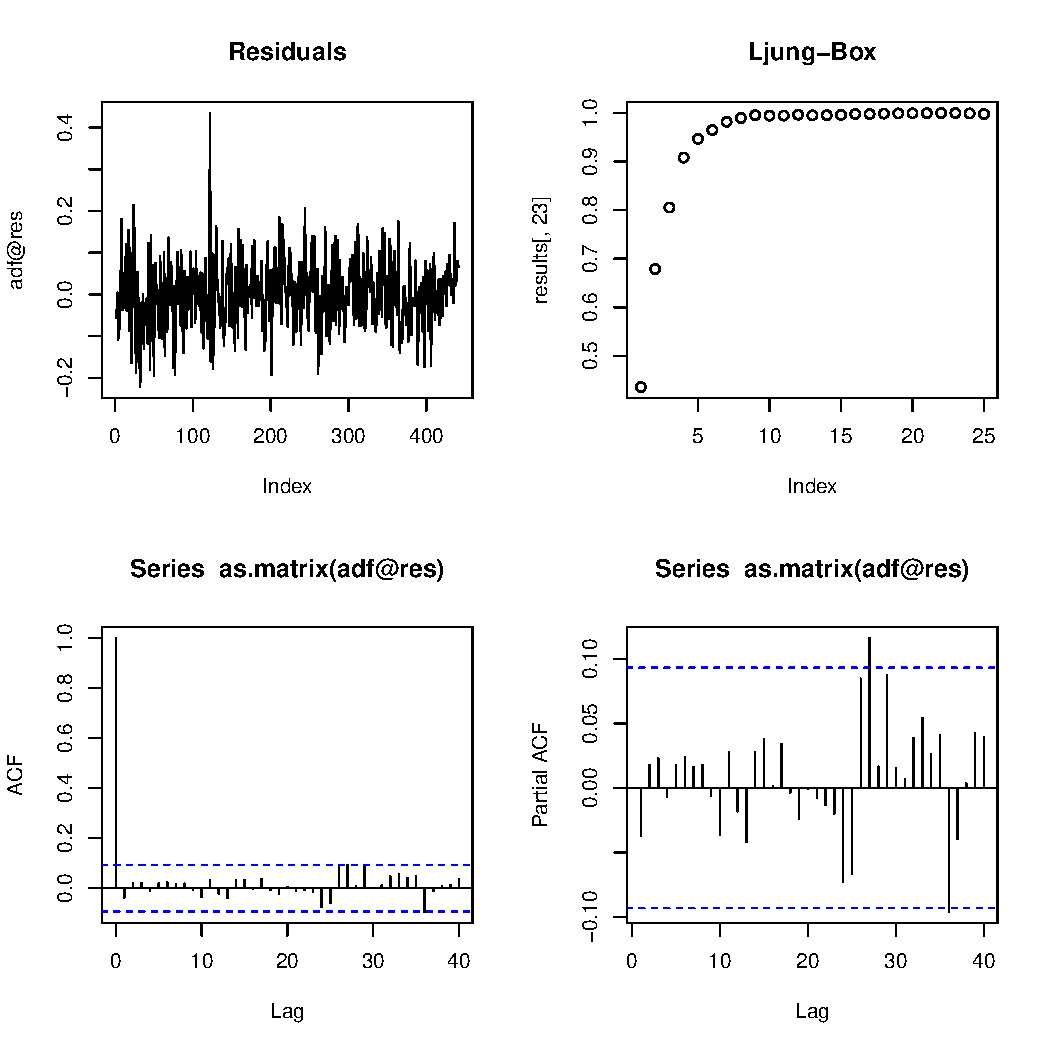
\includegraphics[width=\maxwidth]{figure/unnamed-chunk-51-1} 

\end{knitrout}
            \end{figure}
            
            Tanto o gráfico dos resíduos quanto a sua função de autocorrelação e sua função de autocorrelação parcial indicam que os resíduos se comportam como ruído branco, já que a quantidade de lags significativos é a esperada para um nível de significância de 5\%. o Para testar essa hipótese, realizamos o teste de Ljung-Box para todos os lags até o vinte e cinco. Os testes são realizados no \textit{chunk} abaixo, e na figura abaixo estão os p-valores dos testes para cada lag.
            
\begin{knitrout}
\definecolor{shadecolor}{rgb}{0.969, 0.969, 0.969}\color{fgcolor}\begin{kframe}
\begin{alltt}
\hlstd{boxs} \hlkwb{<-} \hlkwd{all_box}\hlstd{(model1}\hlopt{$}\hlstd{fit}\hlopt{$}\hlstd{residuals)}
\end{alltt}
\end{kframe}
\end{knitrout}

            \begin{figure}[H]
            \caption{P-Valores de Ljung-Box}
            \centering          
\begin{knitrout}
\definecolor{shadecolor}{rgb}{0.969, 0.969, 0.969}\color{fgcolor}\begin{kframe}
\begin{alltt}
\hlkwd{plot}\hlstd{(boxs,} \hlkwc{type}\hlstd{=}\hlstr{'l'}\hlstd{)}
\end{alltt}
\end{kframe}
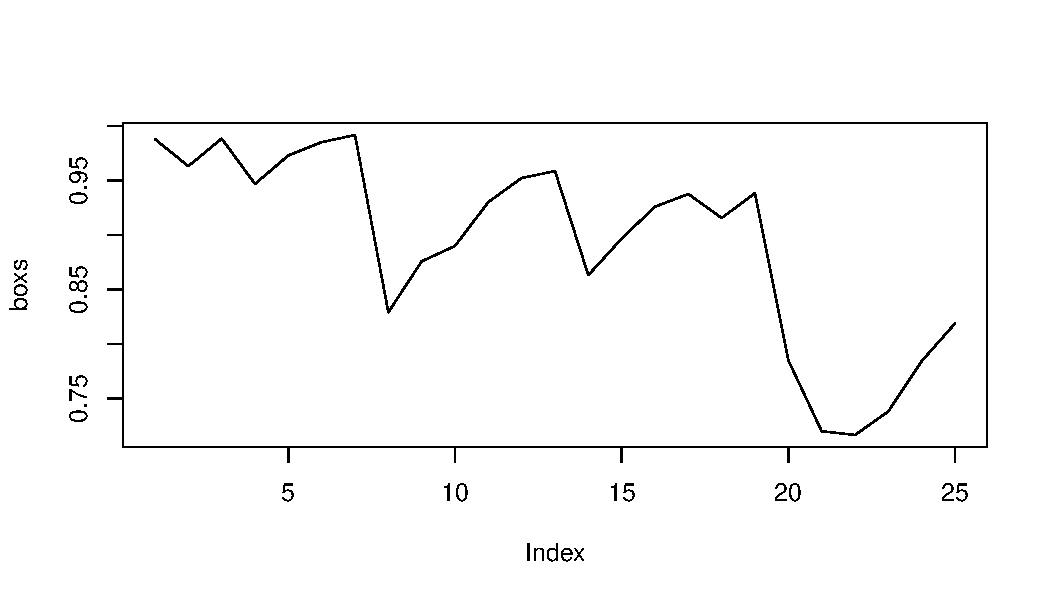
\includegraphics[width=\maxwidth]{figure/unnamed-chunk-53-1} 

\end{knitrout}
            \end{figure}
            
            Abaixo, o valor mínimo do teste de Ljung-Box entre todos os lags considerados.
            
\begin{knitrout}
\definecolor{shadecolor}{rgb}{0.969, 0.969, 0.969}\color{fgcolor}\begin{kframe}
\begin{alltt}
\hlkwd{min}\hlstd{(boxs)}
\end{alltt}
\begin{verbatim}
## [1] 0.7166852
\end{verbatim}
\end{kframe}
\end{knitrout}
            
            Os p-valores não rejeitam a hipótese nula de independência da distribuição, uma vez que todos são superiores a 0,05.
            
        \subsubsection{Homoscedasticidade}
        
            Testamos a homoscedasticidade dos resíduos do modelo selecionado apicando a análise acima nos resíduos ao quadrado.
            
            \begin{figure}[H]
            \caption{Resíduos ao Quadrado}
            \centering
\begin{knitrout}
\definecolor{shadecolor}{rgb}{0.969, 0.969, 0.969}\color{fgcolor}\begin{kframe}
\begin{alltt}
\hlkwd{plot}\hlstd{(model1}\hlopt{$}\hlstd{fit}\hlopt{$}\hlstd{residuals}\hlopt{^}\hlnum{2}\hlstd{)}
\end{alltt}
\end{kframe}
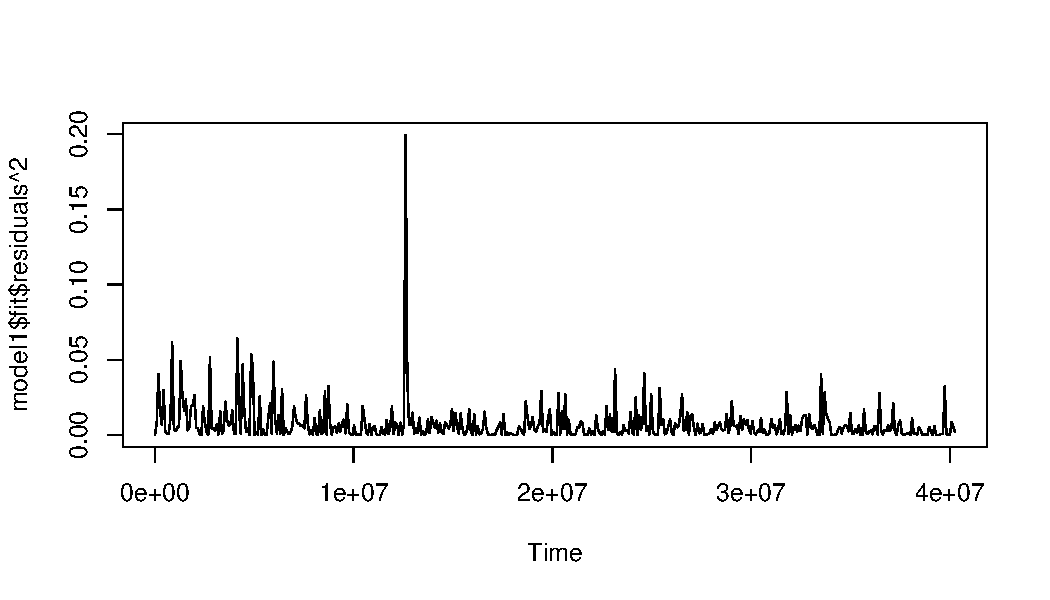
\includegraphics[width=\maxwidth]{figure/unnamed-chunk-55-1} 

\end{knitrout}
            \end{figure}
            
            \begin{figure}[H]
            \caption{FAC dos Resíduos ao Quadrado}
            \centering          
\begin{knitrout}
\definecolor{shadecolor}{rgb}{0.969, 0.969, 0.969}\color{fgcolor}\begin{kframe}
\begin{alltt}
\hlkwd{acf}\hlstd{(}\hlkwd{as.matrix}\hlstd{(model1}\hlopt{$}\hlstd{fit}\hlopt{$}\hlstd{residuals)}\hlopt{^}\hlnum{2}\hlstd{,} \hlkwc{lag.max}\hlstd{=}\hlnum{40}\hlstd{)}
\end{alltt}
\end{kframe}
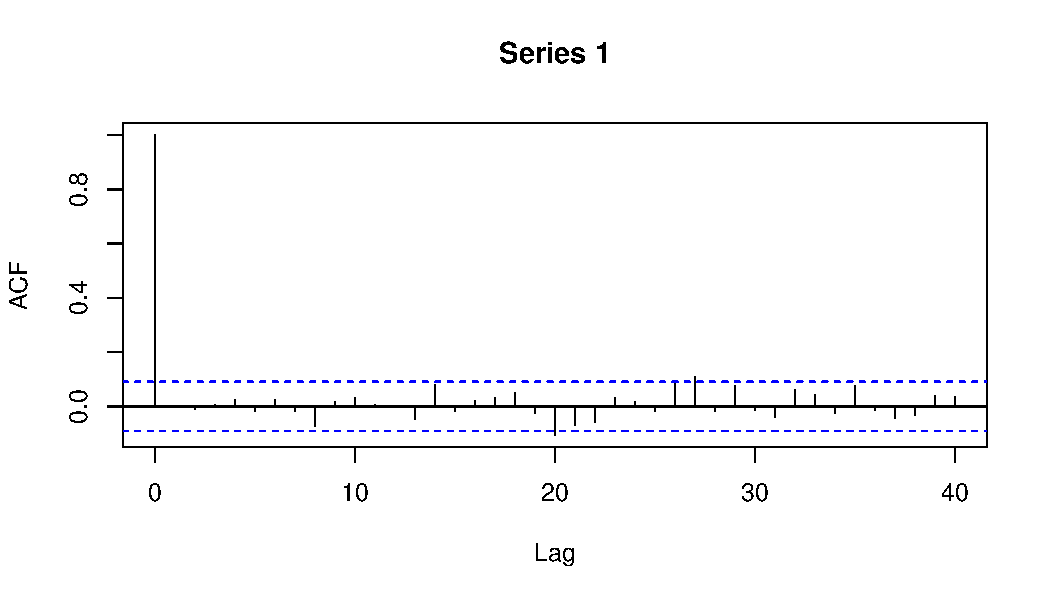
\includegraphics[width=\maxwidth]{figure/unnamed-chunk-56-1} 

\end{knitrout}
            \end{figure}
            
            \begin{figure}[H]
            \caption{FACP dos Resíduos ao Quadrado}
            \centering          
\begin{knitrout}
\definecolor{shadecolor}{rgb}{0.969, 0.969, 0.969}\color{fgcolor}\begin{kframe}
\begin{alltt}
\hlkwd{pacf}\hlstd{(}\hlkwd{as.matrix}\hlstd{(model1}\hlopt{$}\hlstd{fit}\hlopt{$}\hlstd{residuals)}\hlopt{^}\hlnum{2}\hlstd{,} \hlkwc{lag.max}\hlstd{=}\hlnum{40}\hlstd{)}
\end{alltt}
\end{kframe}
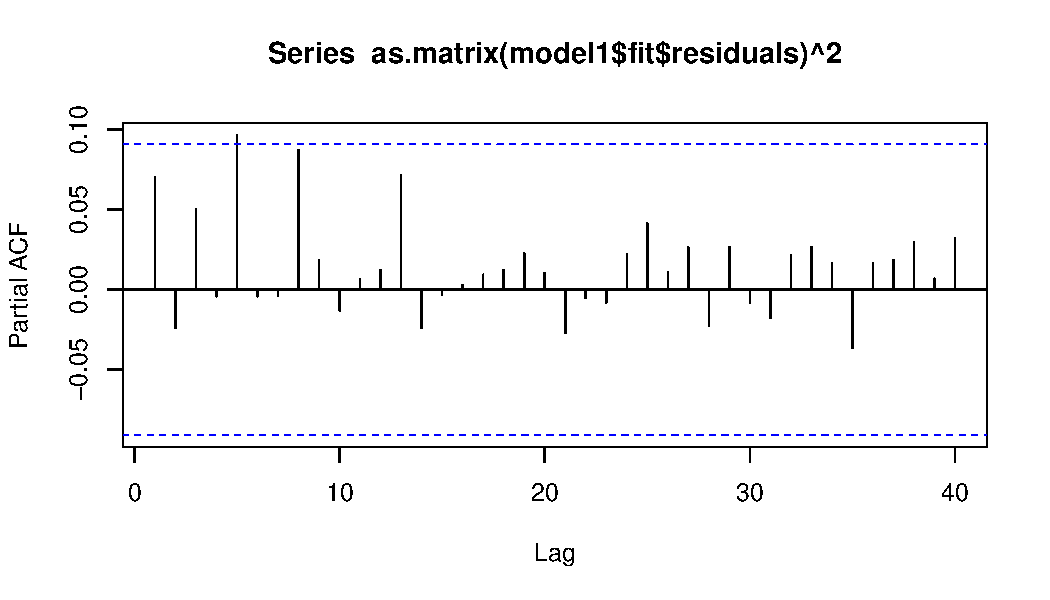
\includegraphics[width=\maxwidth]{figure/unnamed-chunk-57-1} 

\end{knitrout}
            \end{figure}
            
            Tanto o gráfico dos resíduos ao quadrado quanto a sua função de autocorrelação e sua função de autocorrelação parcial indicam homoscedasticidade. Para testar essa hipótese, realizamos o teste de Ljung-Box nos resíduos ao quadrado para todos os lags até o vinte e cinco. Os testes são realizados no \textit{chunk} abaixo, e na figura abaixo estão os p-valores dos testes para cada lag.
            
\begin{knitrout}
\definecolor{shadecolor}{rgb}{0.969, 0.969, 0.969}\color{fgcolor}\begin{kframe}
\begin{alltt}
\hlstd{boxs} \hlkwb{<-} \hlkwd{all_box}\hlstd{(model1}\hlopt{$}\hlstd{fit}\hlopt{$}\hlstd{residuals}\hlopt{^}\hlnum{2}\hlstd{)}
\end{alltt}
\end{kframe}
\end{knitrout}

            \begin{figure}[H]
            \caption{P-Valores de Ljung-Box}
            \centering          
\begin{knitrout}
\definecolor{shadecolor}{rgb}{0.969, 0.969, 0.969}\color{fgcolor}\begin{kframe}
\begin{alltt}
\hlkwd{plot}\hlstd{(boxs,} \hlkwc{type}\hlstd{=}\hlstr{'l'}\hlstd{)}
\end{alltt}
\end{kframe}
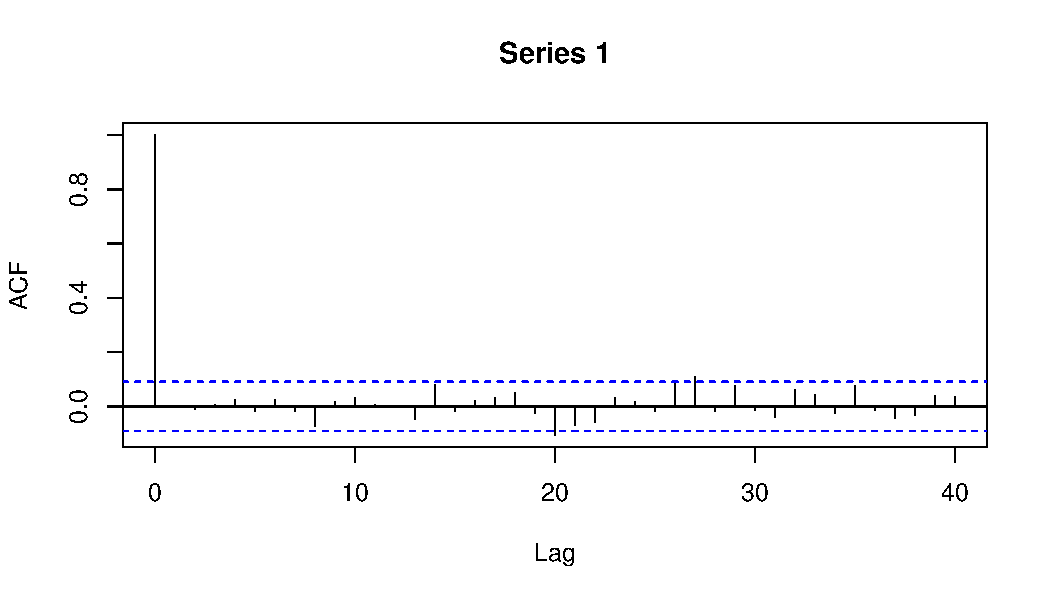
\includegraphics[width=\maxwidth]{figure/unnamed-chunk-59-1} 

\end{knitrout}
            \end{figure}
            
        Abaixo, o valor mínimo do teste de Ljung-Box entre todos os lags considerados.
            
\begin{knitrout}
\definecolor{shadecolor}{rgb}{0.969, 0.969, 0.969}\color{fgcolor}\begin{kframe}
\begin{alltt}
\hlkwd{min}\hlstd{(boxs)}
\end{alltt}
\begin{verbatim}
## [1] 0.1300694
\end{verbatim}
\end{kframe}
\end{knitrout}
            
            Os p-valores não rejeitam a hipótese nula de independência da distribuição. Os resíduos podem ser considerados então homoscedásticos, pois os resíduos ao quadrado são `bem comportados' (ruído branco). Não é necessário então estimar um modelo de variância condicional.


    \subsection{Previsão e Acurácia}
    
        Nesta subseção faremos previsões e testaremos a acurácia das previsões feitas, como passo na avaliação do modelo estimado.
    
        \subsubsection{Previsão}
        
            Agora, realizaremos previsões para os últimos 10 períodos da amostra. Faremos previsão \textit{rolling window}, ou seja: prevemos sempre apenas o período imediatamente subsequente, utilizando a mesma quantidade de dados para todas as previsões.

\begin{knitrout}
\definecolor{shadecolor}{rgb}{0.969, 0.969, 0.969}\color{fgcolor}\begin{kframe}
\begin{alltt}
\hlstd{fs} \hlkwb{<-} \hlkwd{prediction}\hlstd{(data1}\hlopt{$}\hlstd{Value,}\hlnum{2}\hlstd{,}\hlnum{2}\hlstd{,}\hlnum{0}\hlstd{,}\hlnum{2}\hlstd{)}
\end{alltt}
\end{kframe}
\end{knitrout}
  
          Abaixo, as previsões realizadas.

\begin{knitrout}
\definecolor{shadecolor}{rgb}{0.969, 0.969, 0.969}\color{fgcolor}\begin{kframe}
\begin{alltt}
\hlstd{fs}
\end{alltt}
\begin{verbatim}
##  [1] 2.299853 2.082237 2.104396 2.016007 2.085035 2.235921 2.363979 2.474957
##  [9] 2.802898 2.917021
\end{verbatim}
\end{kframe}
\end{knitrout}
          
            Abaixo, os gráficos das previsões e da série original.
        
            \begin{figure}[H]
            \caption{Previsões e Série Original}
            \centering
\begin{knitrout}
\definecolor{shadecolor}{rgb}{0.969, 0.969, 0.969}\color{fgcolor}\begin{kframe}
\begin{alltt}
\hlstd{length} \hlkwb{<-} \hlkwd{length}\hlstd{(data1}\hlopt{$}\hlstd{Value)}
\hlstd{start}  \hlkwb{<-} \hlstd{length} \hlopt{-} \hlnum{9}
\hlstd{series} \hlkwb{<-} \hlstd{data1}\hlopt{$}\hlstd{Value[start}\hlopt{:}\hlstd{length]}
\hlkwd{par}\hlstd{(}\hlkwc{mfrow} \hlstd{=} \hlkwd{c}\hlstd{(}\hlnum{2}\hlstd{,}\hlnum{1}\hlstd{))}
\hlkwd{plot}\hlstd{(fs,}\hlkwc{type}\hlstd{=}\hlstr{'l'}\hlstd{,} \hlkwc{main}\hlstd{=}\hlstr{'Previsões'}\hlstd{)}
\hlkwd{plot}\hlstd{(series)}
\end{alltt}
\end{kframe}
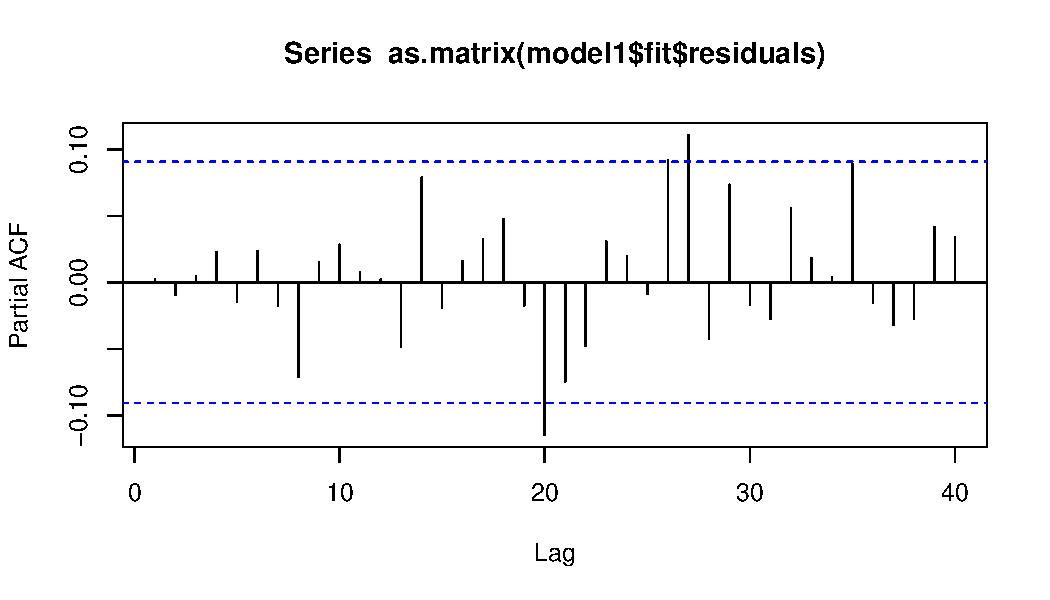
\includegraphics[width=\maxwidth]{figure/unnamed-chunk-62-1} 

\end{knitrout}
            \end{figure}

        \subsubsection{Acurácia}
        
            Agora, vamos calcular a acurácia das previsões. Utilizaremos cinco medidas alternativas: erro médio (ME); erro quadrático médio (RMSE); erro médio absoluto (MAE); erro de porcentagem média (MPE); erro de porcentagem média absoluta (MAPE).
        
\begin{knitrout}
\definecolor{shadecolor}{rgb}{0.969, 0.969, 0.969}\color{fgcolor}\begin{kframe}
\begin{alltt}
\hlkwd{accuracy}\hlstd{(fs,}\hlkwd{as.matrix}\hlstd{(series))}
\end{alltt}
\begin{verbatim}
##                 ME      RMSE       MAE      MPE     MAPE
## Test set 0.1517694 0.2556732 0.2157534 6.290162 8.659937
\end{verbatim}
\end{kframe}
\end{knitrout}

          As medidas acima podem ser úteis na escolha entre modelos, mas não nos dizem muito sobre o modelo se não temos outro para comparar. Para isso usamos o cálculo do Theil's U, que compara as previsões com o que seria uma `adivinhação'. Caso o valor do cálculo for menor que 1, as previsões são melhores que adivinhação. Caso for maior, são piores. O teste é realizado abaixo.
            
\begin{knitrout}
\definecolor{shadecolor}{rgb}{0.969, 0.969, 0.969}\color{fgcolor}\begin{kframe}
\begin{alltt}
\hlkwd{TheilU}\hlstd{(series,fs)}
\end{alltt}
\begin{verbatim}
## [1] 0.1025074
\end{verbatim}
\end{kframe}
\end{knitrout}
        
          O índice do teste foi de 0,102, menor que 1. O modelo fez previsões melhores que uma simples adivinhação.
        



\section{Segunda Parte da Série Temporal}

    \subsection{Definição da Ordem de Integração}
    
        O primeiro passo na metodologia Box-Jenkins (\cite{boxjenkins}) é a definição da ordem de integração da série temporal .
    
        \subsubsection{Análise da Série Original}
        
            Começamos o processo de definição da ordem de integração analisando o gráfico da série temporal.
        
            \begin{figure}[H]
            \caption{Série Temporal}
            \centering
\begin{knitrout}
\definecolor{shadecolor}{rgb}{0.969, 0.969, 0.969}\color{fgcolor}\begin{kframe}
\begin{alltt}
\hlkwd{plot}\hlstd{(data2)}
\end{alltt}
\end{kframe}
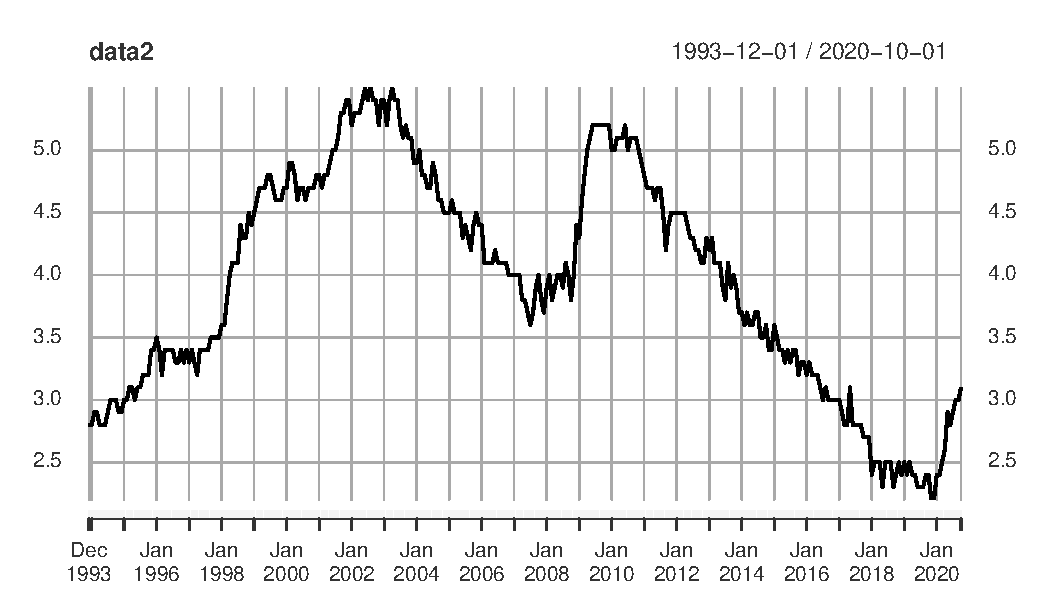
\includegraphics[width=\maxwidth]{figure/unnamed-chunk-65-1} 

\end{knitrout}
            \end{figure}
            
            O gráfico assemelha-se a um passeio aleatório, portanto, indicandio a presença de raíz unitária. Para coletar mais indícios visuais analisamos abaixo a função de autocorrelação e a fução de autocorrelação parcial.
            
            \begin{figure}[H]
            \caption{FAC da Série Temporal}
            \centering
\begin{knitrout}
\definecolor{shadecolor}{rgb}{0.969, 0.969, 0.969}\color{fgcolor}\begin{kframe}
\begin{alltt}
\hlkwd{acf}\hlstd{(}\hlkwd{as.matrix}\hlstd{(data2),} \hlkwc{lag.max}\hlstd{=}\hlnum{60}\hlstd{)}
\end{alltt}
\end{kframe}
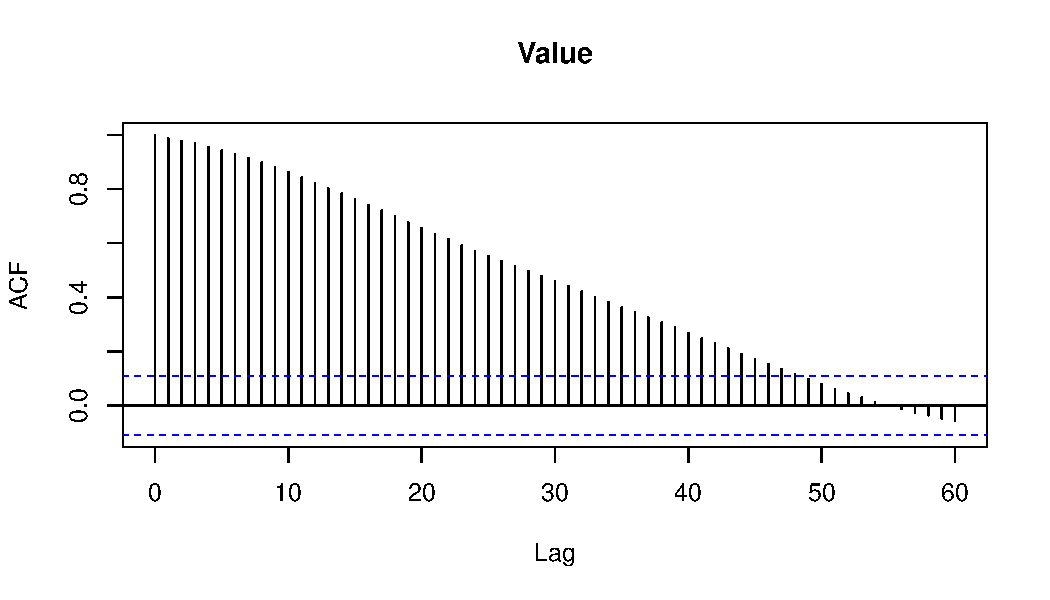
\includegraphics[width=\maxwidth]{figure/unnamed-chunk-66-1} 

\end{knitrout}
            \end{figure}
            
            \begin{figure}[H]
            \caption{FACP da Série Temporal}
            \centering
\begin{knitrout}
\definecolor{shadecolor}{rgb}{0.969, 0.969, 0.969}\color{fgcolor}\begin{kframe}
\begin{alltt}
\hlkwd{pacf}\hlstd{(}\hlkwd{as.matrix}\hlstd{(data2),} \hlkwc{lag.max}\hlstd{=}\hlnum{60}\hlstd{)}
\end{alltt}
\end{kframe}
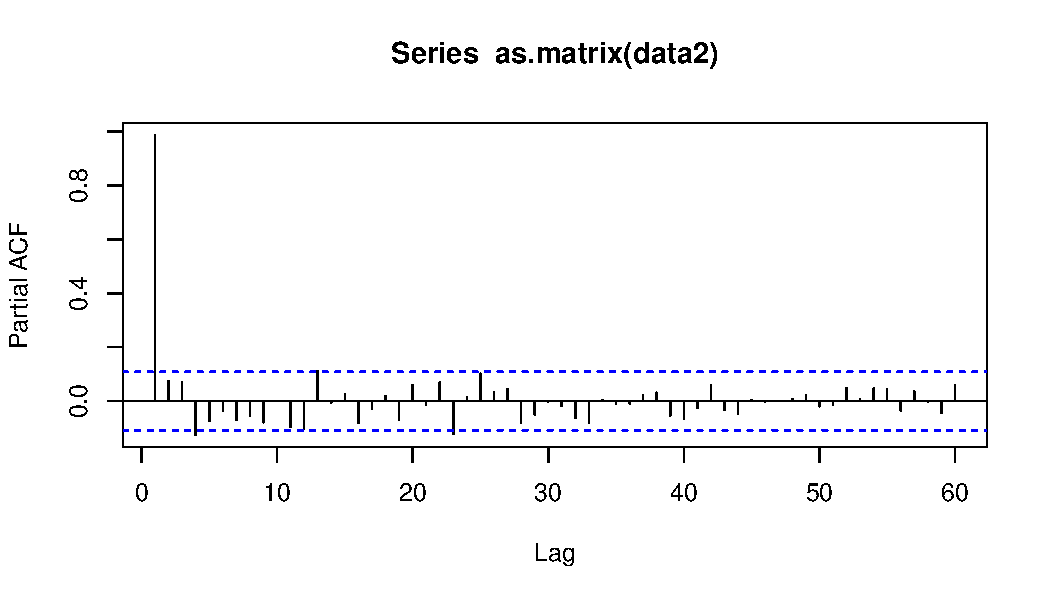
\includegraphics[width=\maxwidth]{figure/unnamed-chunk-67-1} 

\end{knitrout}
            \end{figure}
            
            A função de autocorrelação aparentemente possui decaimento lento, indicando possibilidade de raiz unitária. Para testar a hipótese de presença de raiz unitária com o teste Dickey-Fuller aumentado (\cite{adf}). O teste será realizado sem \textit{drift} ou tendência, pois a visualização do gráfico da série temporal não indica a presença de tais. Para escolher o lag do teste, começaremos pelo lag 1 e, caso os resíduos do teste forem ruído branco, aceitamos o lag. Caso os resíduos não apresentarem comportamento de ruído branco, repetimos os passos com o lag imediatamente maior. No \textit{chunk} abaixo realizamos testes ADF para 24 lags, e para cada teste testamos os resíduos com testes de Ljung-Box (\cite{ljungbox}) até 25 lags.

\begin{knitrout}
\definecolor{shadecolor}{rgb}{0.969, 0.969, 0.969}\color{fgcolor}\begin{kframe}
\begin{alltt}
\hlstd{lag} \hlkwb{<-} \hlkwd{select_adf}\hlstd{(data2}\hlopt{$}\hlstd{Value,} \hlstr{"none"}\hlstd{)}
\hlstd{lag}
\end{alltt}
\begin{verbatim}
## [1] 14
\end{verbatim}
\end{kframe}
\end{knitrout}

            Escolhemos a ordem de lag 14.

\begin{knitrout}
\definecolor{shadecolor}{rgb}{0.969, 0.969, 0.969}\color{fgcolor}\begin{kframe}
\begin{alltt}
\hlstd{adf} \hlkwb{<-} \hlkwd{ur.df}\hlstd{(}\hlkwd{na.omit}\hlstd{(data2}\hlopt{$}\hlstd{Value),} \hlstr{"none"}\hlstd{,} \hlkwc{lags}\hlstd{=lag)}
\end{alltt}
\end{kframe}
\end{knitrout}

            \begin{figure}[H]
            \caption{Resíduos}
            \centering
\begin{knitrout}
\definecolor{shadecolor}{rgb}{0.969, 0.969, 0.969}\color{fgcolor}\begin{kframe}
\begin{alltt}
\hlkwd{par}\hlstd{(}\hlkwc{mfrow} \hlstd{=} \hlkwd{c}\hlstd{(}\hlnum{2}\hlstd{,}\hlnum{2}\hlstd{))}
\hlkwd{plot}\hlstd{(adf}\hlopt{@}\hlkwc{res}\hlstd{,} \hlkwc{type}\hlstd{=}\hlstr{'l'}\hlstd{,} \hlkwc{main}\hlstd{=}\hlstr{'Residuals'}\hlstd{)}
\hlkwd{plot}\hlstd{(}\hlkwd{all_box}\hlstd{(adf}\hlopt{@}\hlkwc{res}\hlstd{),} \hlkwc{main}\hlstd{=}\hlstr{'Ljung-Box'}\hlstd{)}
\hlkwd{acf}\hlstd{(}\hlkwd{as.matrix}\hlstd{(adf}\hlopt{@}\hlkwc{res}\hlstd{),} \hlkwc{lag.max}\hlstd{=}\hlnum{60}\hlstd{)}
\hlkwd{pacf}\hlstd{(}\hlkwd{as.matrix}\hlstd{(adf}\hlopt{@}\hlkwc{res}\hlstd{),} \hlkwc{lag.max}\hlstd{=}\hlnum{60}\hlstd{)}
\end{alltt}
\end{kframe}
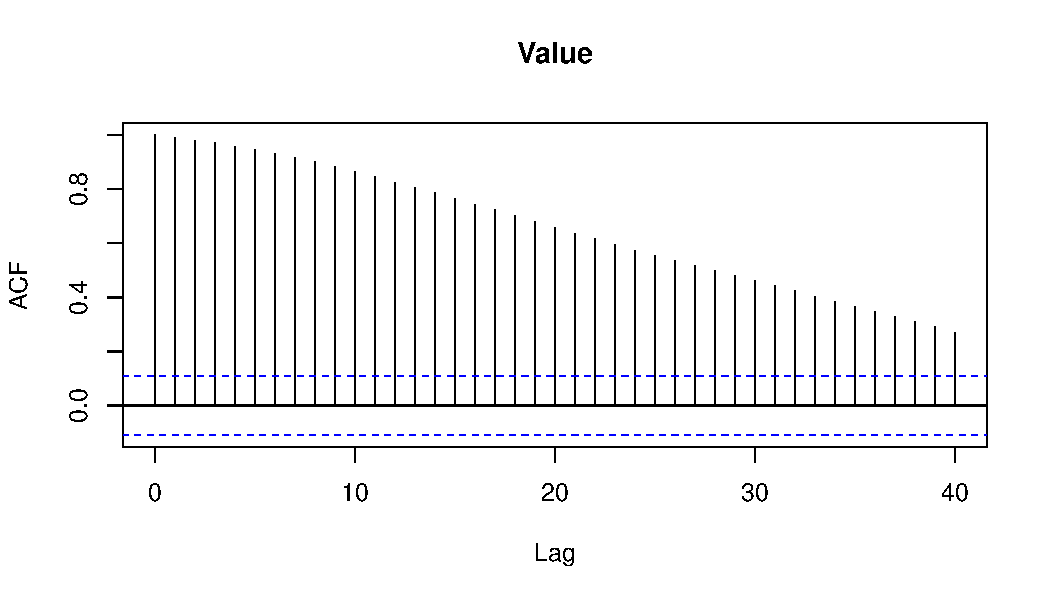
\includegraphics[width=\maxwidth]{figure/unnamed-chunk-70-1} 

\end{knitrout}
            \end{figure}

            Tanto o gráfico dos resíduos quanto os gráficos das funções de autocorrelação e autocorrelação parcial indicam que os resíduos do teste se comportam como ruído branco. Os p-valores do teste de Ljung-Box não rejeitam a hipótese de independência dos resíduos.
            
            Agora, visualizamos as estatísticas do teste e os valores críticos        
            
\begin{knitrout}
\definecolor{shadecolor}{rgb}{0.969, 0.969, 0.969}\color{fgcolor}\begin{kframe}
\begin{alltt}
\hlstd{adf}\hlopt{@}\hlkwc{teststat}
\end{alltt}
\begin{verbatim}
##                 tau1
## statistic -0.2342756
\end{verbatim}
\begin{alltt}
\hlstd{adf}\hlopt{@}\hlkwc{cval}
\end{alltt}
\begin{verbatim}
##       1pct  5pct 10pct
## tau1 -2.58 -1.95 -1.62
\end{verbatim}
\end{kframe}
\end{knitrout}

            O valor da estatística do teste é de -0.2343. Os valores críticos para o teste são de -2,58 (1\%), -1,95 (5\%) e -1,62 (10\%). Sendo assim, o valor do teste não ultrapassou os valores críticos para nenhum grau de significância. O teste então aceita a hipótese nula de presença de raiz unitária.

        \subsubsection{Diferenciação}
        
            Como tentativa para estacionarizar a série, aplicamos a primeira diferença.

\begin{knitrout}
\definecolor{shadecolor}{rgb}{0.969, 0.969, 0.969}\color{fgcolor}\begin{kframe}
\begin{alltt}
\hlstd{data2}\hlopt{$}\hlstd{Diff} \hlkwb{<-} \hlkwd{diff}\hlstd{(data2)}
\end{alltt}
\end{kframe}
\end{knitrout}

            Abaixo, o sumário dos novos dados.
            
\begin{knitrout}
\definecolor{shadecolor}{rgb}{0.969, 0.969, 0.969}\color{fgcolor}\begin{kframe}
\begin{alltt}
\hlkwd{summary}\hlstd{(data2)}
\end{alltt}
\begin{verbatim}
##      Index                         Value            Diff           
##  Min.   :1993-12-01 00:00:00   Min.   :2.200   Min.   :-0.3000000  
##  1st Qu.:2000-08-16 12:00:00   1st Qu.:3.200   1st Qu.:-0.1000000  
##  Median :2007-05-01 00:00:00   Median :4.000   Median : 0.0000000  
##  Mean   :2007-05-02 04:00:44   Mean   :3.948   Mean   : 0.0009317  
##  3rd Qu.:2014-01-16 12:00:00   3rd Qu.:4.700   3rd Qu.: 0.1000000  
##  Max.   :2020-10-01 00:00:00   Max.   :5.500   Max.   : 0.4000000  
##                                                NA's   :1
\end{verbatim}
\end{kframe}
\end{knitrout}
      
        \subsubsection{Análise da Primeira Diferença}
        
            Começamos a nova análise analisando o gráfico da primeira diferença da série temporal.
        
            \begin{figure}[H]
            \caption{Primeira Diferença}
            \centering
\begin{knitrout}
\definecolor{shadecolor}{rgb}{0.969, 0.969, 0.969}\color{fgcolor}\begin{kframe}
\begin{alltt}
\hlkwd{plot}\hlstd{(data2}\hlopt{$}\hlstd{Diff)}
\end{alltt}
\end{kframe}
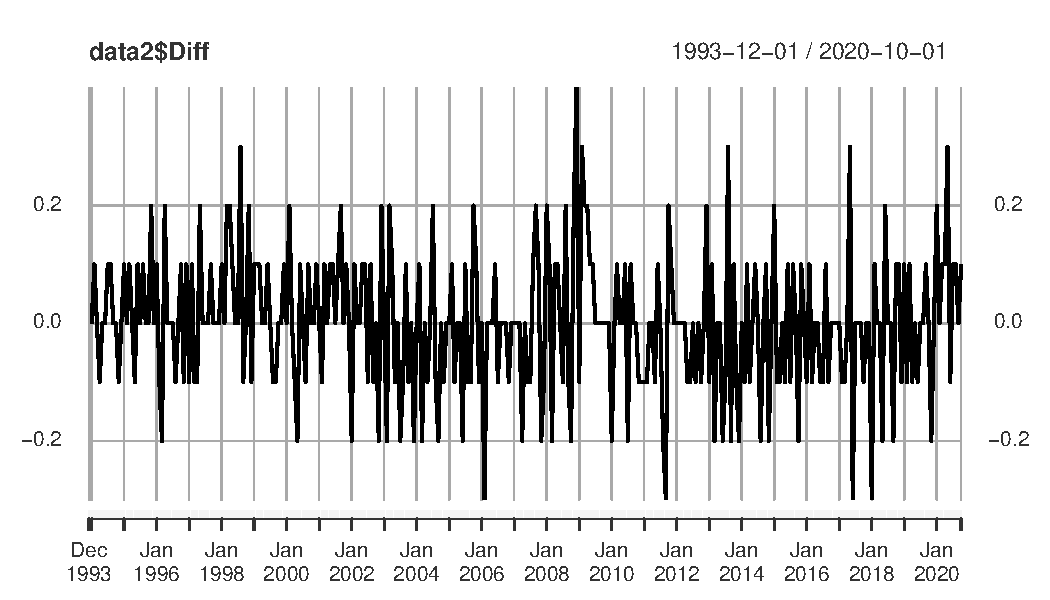
\includegraphics[width=\maxwidth]{figure/unnamed-chunk-74-1} 

\end{knitrout}
            \end{figure}
            
            A analise visual do gráfico sugere variação em torno de uma média sem distanciamento grande por longos períodos, portanto, indica que a estacionariedade da série foi obtida na primeira diferenciação.
            
            \begin{figure}[H]
            \caption{FAC da Primeira Diferença}
            \centering
\begin{knitrout}
\definecolor{shadecolor}{rgb}{0.969, 0.969, 0.969}\color{fgcolor}\begin{kframe}
\begin{alltt}
\hlkwd{acf}\hlstd{(}\hlkwd{as.matrix}\hlstd{(}\hlkwd{na.omit}\hlstd{(data2}\hlopt{$}\hlstd{Diff)),} \hlkwc{lag.max}\hlstd{=}\hlnum{60}\hlstd{)}
\end{alltt}
\end{kframe}
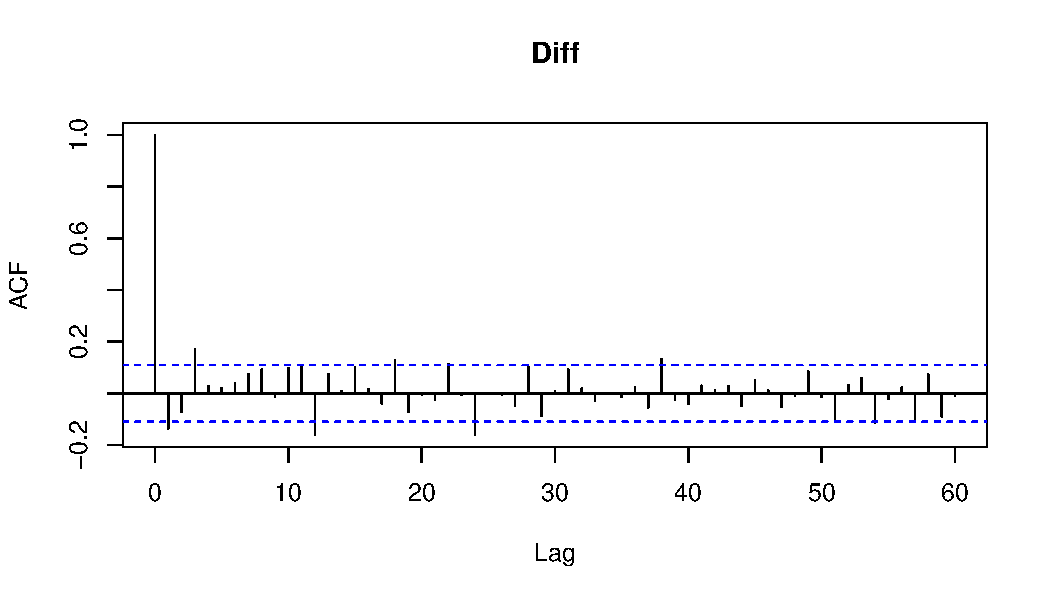
\includegraphics[width=\maxwidth]{figure/unnamed-chunk-75-1} 

\end{knitrout}
            \end{figure}
            
            \begin{figure}[H]
            \caption{FACP da Primeira Diferença}
            \centering
\begin{knitrout}
\definecolor{shadecolor}{rgb}{0.969, 0.969, 0.969}\color{fgcolor}\begin{kframe}
\begin{alltt}
\hlkwd{pacf}\hlstd{(}\hlkwd{as.matrix}\hlstd{(}\hlkwd{na.omit}\hlstd{(data2}\hlopt{$}\hlstd{Diff)),} \hlkwc{lag.max}\hlstd{=}\hlnum{60}\hlstd{)}
\end{alltt}
\end{kframe}
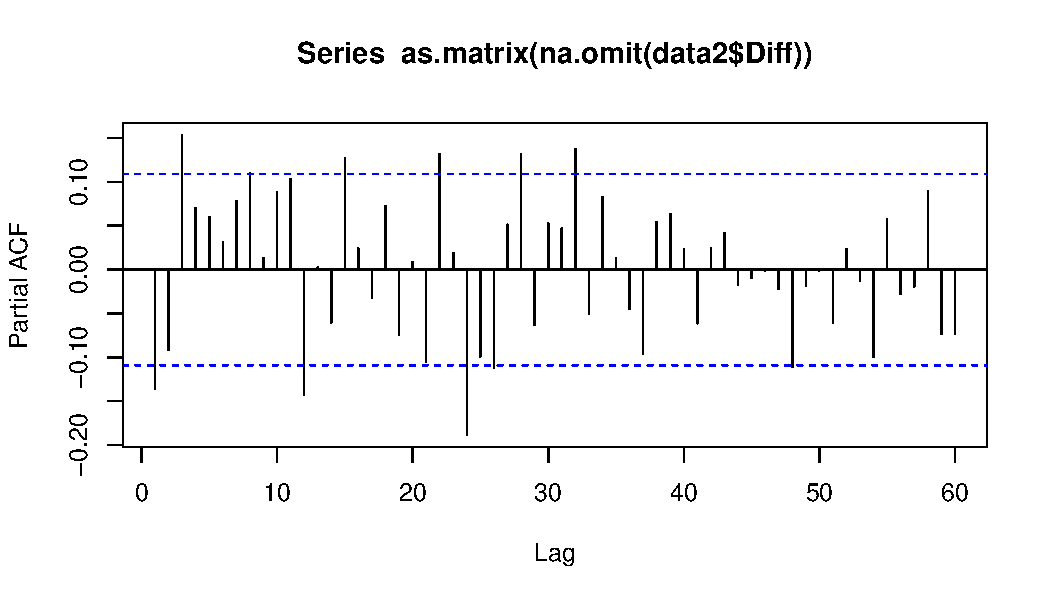
\includegraphics[width=\maxwidth]{figure/unnamed-chunk-76-1} 

\end{knitrout}
            \end{figure}
            
            A análise dos gráficos pós diferenciação indica rápido decaimento nas funções ACF e PACF, reforçando a hipótese de que não há raíz unitária. Agora testaremos, com o teste de Dickey-Fuller aumentado, a presença de raiz unitária. Não adicionaremos drift ou tendância no teste pois não há indício pelo gráfico da série de existência de algum desses parâmetros. Seguiremos os passos descritos acima, quando aplicamos o teste na série temporal original.
            
\begin{knitrout}
\definecolor{shadecolor}{rgb}{0.969, 0.969, 0.969}\color{fgcolor}\begin{kframe}
\begin{alltt}
\hlstd{lag} \hlkwb{<-} \hlkwd{select_adf}\hlstd{(}\hlkwd{na.omit}\hlstd{(data2}\hlopt{$}\hlstd{Diff),}\hlstr{"none"}\hlstd{)}
\hlstd{lag}
\end{alltt}
\begin{verbatim}
## [1] 13
\end{verbatim}
\end{kframe}
\end{knitrout}

            Escolhemos a ordem de lag 13.

\begin{knitrout}
\definecolor{shadecolor}{rgb}{0.969, 0.969, 0.969}\color{fgcolor}\begin{kframe}
\begin{alltt}
\hlstd{adf} \hlkwb{<-} \hlkwd{ur.df}\hlstd{(}\hlkwd{na.omit}\hlstd{(data2}\hlopt{$}\hlstd{Diff),} \hlkwc{lags}\hlstd{=lag)}
\end{alltt}
\end{kframe}
\end{knitrout}

            \begin{figure}[H]
            \caption{Resíduos}
            \centering
\begin{knitrout}
\definecolor{shadecolor}{rgb}{0.969, 0.969, 0.969}\color{fgcolor}\begin{kframe}
\begin{alltt}
\hlkwd{par}\hlstd{(}\hlkwc{mfrow} \hlstd{=} \hlkwd{c}\hlstd{(}\hlnum{2}\hlstd{,}\hlnum{2}\hlstd{))}
\hlkwd{plot}\hlstd{(adf}\hlopt{@}\hlkwc{res}\hlstd{,} \hlkwc{type}\hlstd{=}\hlstr{'l'}\hlstd{,} \hlkwc{main}\hlstd{=}\hlstr{'Residuals'}\hlstd{)}
\hlkwd{plot}\hlstd{(}\hlkwd{all_box}\hlstd{(adf}\hlopt{@}\hlkwc{res}\hlstd{),} \hlkwc{main}\hlstd{=}\hlstr{'Ljung-Box'}\hlstd{)}
\hlkwd{acf}\hlstd{(}\hlkwd{as.matrix}\hlstd{(adf}\hlopt{@}\hlkwc{res}\hlstd{),} \hlkwc{lag.max}\hlstd{=}\hlnum{60}\hlstd{)}
\hlkwd{pacf}\hlstd{(}\hlkwd{as.matrix}\hlstd{(adf}\hlopt{@}\hlkwc{res}\hlstd{),} \hlkwc{lag.max}\hlstd{=}\hlnum{60}\hlstd{)}
\end{alltt}
\end{kframe}
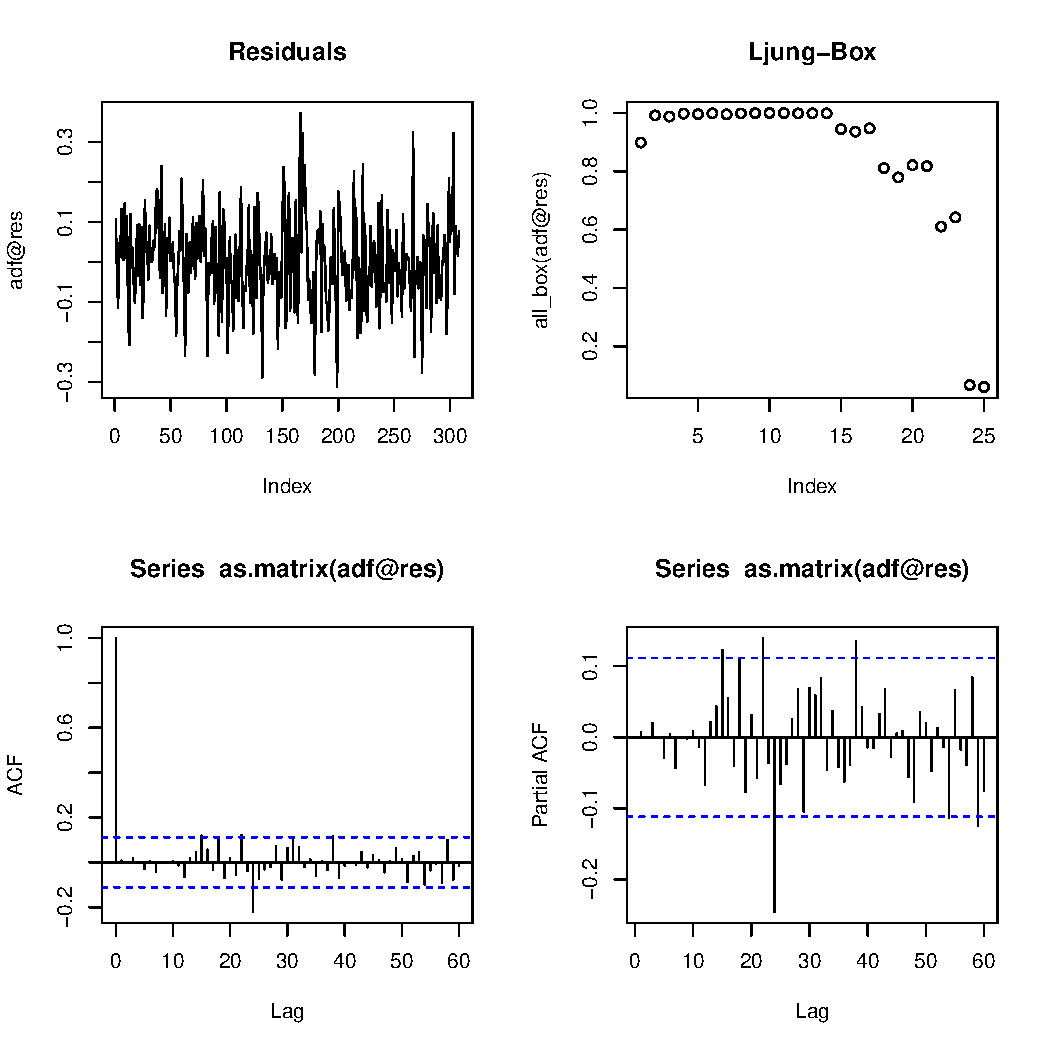
\includegraphics[width=\maxwidth]{figure/unnamed-chunk-79-1} 

\end{knitrout}
            \end{figure}

            Tanto o gráfico dos resíduos quanto os gráficos das funções de autocorrelação e autocorrelação parcial indicam que os resíduos do teste se comportam como ruído branco. Os p-valores do teste de Ljung-Box não rejeitam a hipótese de independência dos resíduos.
            
            Agora, visualizamos as estatísticas do teste e os valores críticos        
            
\begin{knitrout}
\definecolor{shadecolor}{rgb}{0.969, 0.969, 0.969}\color{fgcolor}\begin{kframe}
\begin{alltt}
\hlstd{adf}\hlopt{@}\hlkwc{teststat}
\end{alltt}
\begin{verbatim}
##                tau1
## statistic -3.491532
\end{verbatim}
\begin{alltt}
\hlstd{adf}\hlopt{@}\hlkwc{cval}
\end{alltt}
\begin{verbatim}
##       1pct  5pct 10pct
## tau1 -2.58 -1.95 -1.62
\end{verbatim}
\end{kframe}
\end{knitrout}

            O valor da estatística do teste é de 3,4915. Os valores críticos para o teste são de -2,58 (1\%), -1,95 (5\%) e -1,62 (10\%). Sendo assim, o valor do teste ultrapassou os valores críticos para todos os graus de significância. O teste então rejeita a hipótese nula de presença de raiz unitária. O resultado obtido é, então, que a série temporal original é integrada de ordem um - I(1).
            
            
        \subsubsection{Diferença Sazonal}
    
            A função de autocorrelação indica que existem lags sazonais significativos, no entando, o decaimento é rápido, indicanco não existência de raiz unitária sazonal.Testamos a seguir a hipótese nula de não presença de raiz unitária sazonal com o teste de Canova e Hansen (\cite{ch}).
          
\begin{knitrout}
\definecolor{shadecolor}{rgb}{0.969, 0.969, 0.969}\color{fgcolor}\begin{kframe}
\begin{alltt}
\hlstd{ch} \hlkwb{=} \hlkwd{ch.test}\hlstd{(}\hlkwd{ts}\hlstd{(}\hlkwd{na.omit}\hlstd{(data2}\hlopt{$}\hlstd{Diff),} \hlkwc{frequency}\hlstd{=}\hlnum{12}\hlstd{),} \hlkwc{type}\hlstd{=}\hlstr{"dummy"}\hlstd{,} \hlkwc{sid}\hlstd{=}\hlkwd{c}\hlstd{(}\hlnum{1}\hlopt{:}\hlnum{12}\hlstd{))}
\hlstd{ch}\hlopt{$}\hlstd{pvalues}
\end{alltt}
\begin{verbatim}
## [1] 0.6117258
\end{verbatim}
\end{kframe}
\end{knitrout}

            O teste retornou um p-valor de 0.6117, o que significa que não podemos rejeitar a hipótese nula de não presença de raiz unitária sazonal.


    \subsection{Identificação das Possíveis Formas Funcionais}
    
        \begin{figure}[H]
        \caption{FAC da Primeira Diferença}
        \centering
\begin{knitrout}
\definecolor{shadecolor}{rgb}{0.969, 0.969, 0.969}\color{fgcolor}\begin{kframe}
\begin{alltt}
\hlkwd{acf}\hlstd{(}\hlkwd{as.matrix}\hlstd{(}\hlkwd{na.omit}\hlstd{(data2}\hlopt{$}\hlstd{Diff)),} \hlkwc{lag.max}\hlstd{=}\hlnum{60}\hlstd{)}
\end{alltt}
\end{kframe}
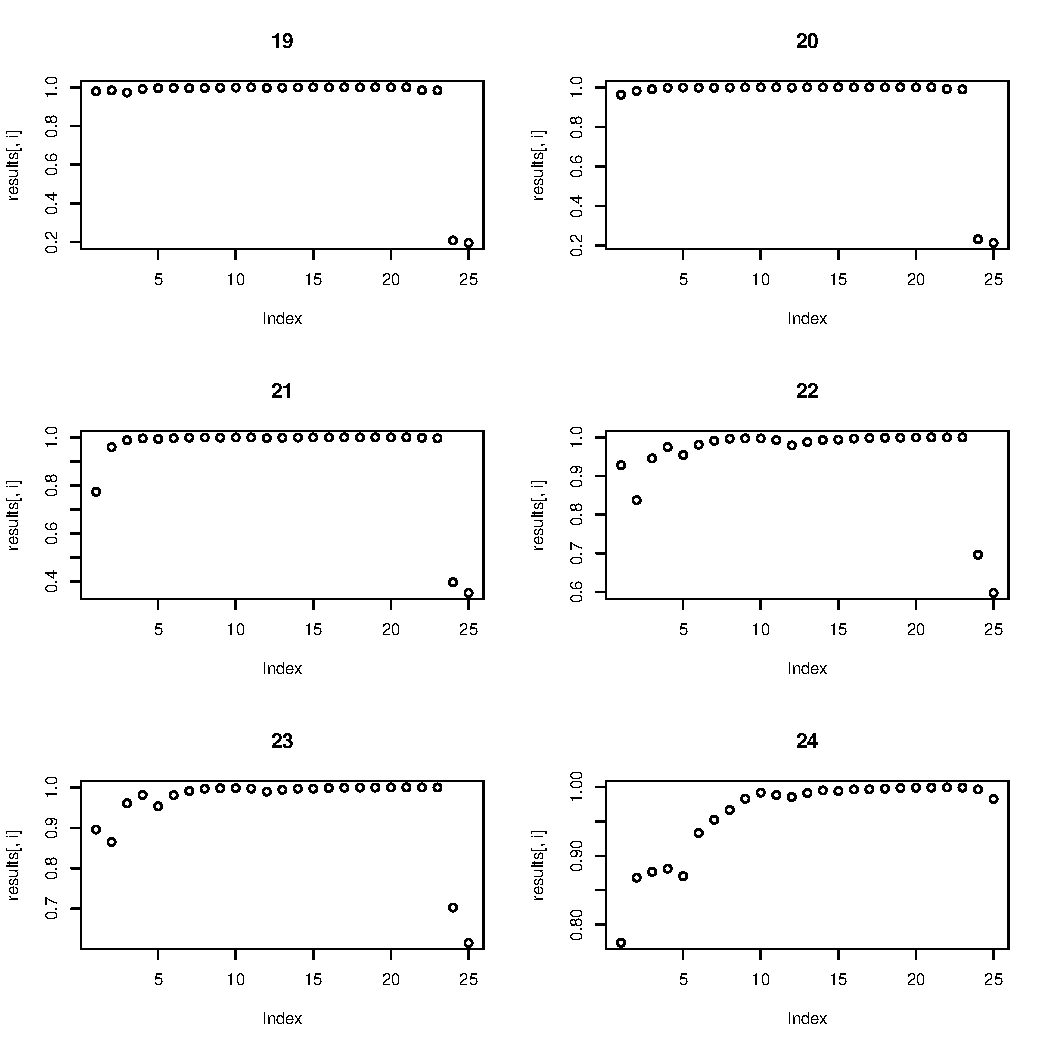
\includegraphics[width=\maxwidth]{figure/unnamed-chunk-82-1} 

\end{knitrout}
        \end{figure}
        
        A função de autocorrelação tem até o terceiro lag significativo, enquanto mostra dois lags significativo no fator sazonal.
        
        \begin{figure}[H]
        \caption{FACP da Primeira Diferença}
        \centering
\begin{knitrout}
\definecolor{shadecolor}{rgb}{0.969, 0.969, 0.969}\color{fgcolor}\begin{kframe}
\begin{alltt}
\hlkwd{pacf}\hlstd{(}\hlkwd{as.matrix}\hlstd{(}\hlkwd{na.omit}\hlstd{(data2}\hlopt{$}\hlstd{Diff)),} \hlkwc{lag.max}\hlstd{=}\hlnum{60}\hlstd{)}
\end{alltt}
\end{kframe}
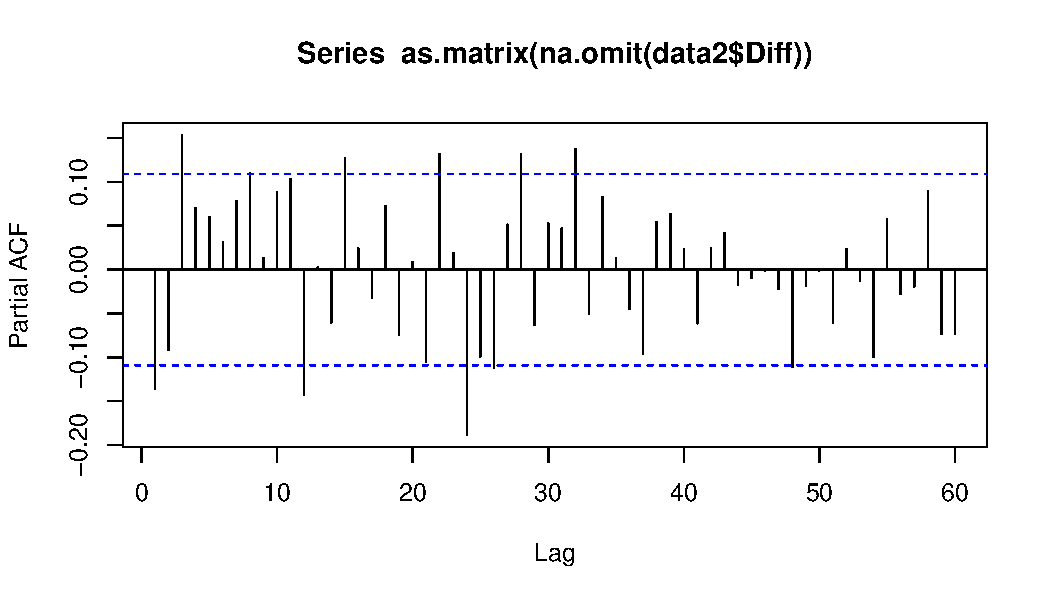
\includegraphics[width=\maxwidth]{figure/unnamed-chunk-83-1} 

\end{knitrout}
        \end{figure}

        A função de autocorrelação parcial tem até o terceiro lag significativo, enquanto mostra dois lags significativos no fator sazonal.
        
        A análise das funções acima sugere que uma ordem máxima para o modelo SARIMA é (3,1,3)(2,0,2)12.


    \subsection{Estimação}
    
        Na subseção anterior definimos as ordems máximas do modelo SARIMA. Nesta seção vamos estimar todos os modelos até as ordens máximas, testar seus resíduos para checar se comportam-se como ruído branco e, finalmente, escolher os modelos que passam o teste dos resíduos que apresentam melhores critérios de informação (AIC e BIC). Esses passos são realizados no \textit{chunk} abaixo.


\begin{knitrout}
\definecolor{shadecolor}{rgb}{0.969, 0.969, 0.969}\color{fgcolor}\begin{kframe}
\begin{alltt}
\hlstd{order} \hlkwb{<-} \hlkwd{select_model}\hlstd{(data2}\hlopt{$}\hlstd{Value,}\hlnum{3}\hlstd{,}\hlnum{1}\hlstd{,}\hlnum{3}\hlstd{,}\hlnum{2}\hlstd{,}\hlnum{0}\hlstd{,}\hlnum{2}\hlstd{,}\hlnum{12}\hlstd{)}
\end{alltt}
\end{kframe}
\end{knitrout}

        Abaixo, as ordens dos melhores modelos pelos critérios AIC e BIC.

\begin{knitrout}
\definecolor{shadecolor}{rgb}{0.969, 0.969, 0.969}\color{fgcolor}\begin{kframe}
\begin{alltt}
\hlcom{# Ordem pelo critério AIC}
\hlkwd{print}\hlstd{(}\hlstr{"p q P Q"}\hlstd{)}
\end{alltt}
\begin{verbatim}
## [1] "p q P Q"
\end{verbatim}
\begin{alltt}
\hlstd{order[,}\hlnum{1}\hlstd{]}
\end{alltt}
\begin{verbatim}
## [1] 3 1 0 2
\end{verbatim}
\begin{alltt}
\hlcom{# Ordem pelo critério BIC}
\hlkwd{print}\hlstd{(}\hlstr{"p q P Q"}\hlstd{)}
\end{alltt}
\begin{verbatim}
## [1] "p q P Q"
\end{verbatim}
\begin{alltt}
\hlstd{order[,}\hlnum{2}\hlstd{]}
\end{alltt}
\begin{verbatim}
## [1] 1 2 0 2
\end{verbatim}
\end{kframe}
\end{knitrout}

        O modelo com melhor critério AIC é o SARIMA (3,1,1)(0,0,2)12. O modelo com melhor critério BIC é o SARIMA (1,1,2)(0,0,2)12. Pelo critério da parcimônia selecionamos o modelo com melhor critério BIC, pois é o que apresenta menor quantidade de parâmetros.
            
\begin{knitrout}
\definecolor{shadecolor}{rgb}{0.969, 0.969, 0.969}\color{fgcolor}\begin{kframe}
\begin{alltt}
\hlstd{model2} \hlkwb{<-} \hlkwd{sarima}\hlstd{(data2}\hlopt{$}\hlstd{Value,}
                \hlnum{1}\hlstd{,} \hlnum{1}\hlstd{,} \hlnum{2}\hlstd{,}
                \hlnum{0}\hlstd{,} \hlnum{0}\hlstd{,} \hlnum{2}\hlstd{,} \hlnum{12}\hlstd{)}
\end{alltt}
\end{kframe}
\end{knitrout}


    \subsection{Diagnóstico dos Resíduos}
    
        Nesta seção iremos fazer o diagnóstico dos resíduos. Para isso vamos analisar sua independência e homoscedasticidade.

        \subsubsection{Independência}
        
            Para analisar a independência dos resíduos analisamos o gráfico dos resíduos, a função de autocorrelação e a função de autocorrelação parcial.
        
            \begin{figure}[H]
            \caption{Resíduos}
            \centering
\begin{knitrout}
\definecolor{shadecolor}{rgb}{0.969, 0.969, 0.969}\color{fgcolor}\begin{kframe}
\begin{alltt}
\hlkwd{plot}\hlstd{(model2}\hlopt{$}\hlstd{fit}\hlopt{$}\hlstd{residuals)}
\end{alltt}
\end{kframe}
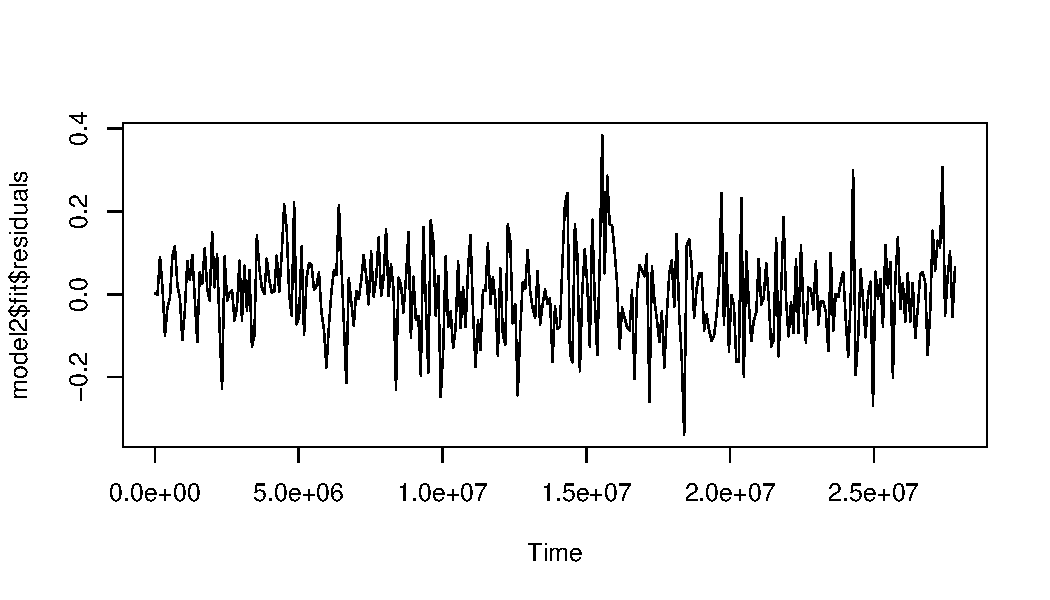
\includegraphics[width=\maxwidth]{figure/unnamed-chunk-85-1} 

\end{knitrout}
            \end{figure}
            
            \begin{figure}[H]
            \caption{FAC dos Resíduos}
            \centering          
\begin{knitrout}
\definecolor{shadecolor}{rgb}{0.969, 0.969, 0.969}\color{fgcolor}\begin{kframe}
\begin{alltt}
\hlkwd{acf}\hlstd{(}\hlkwd{as.matrix}\hlstd{(model2}\hlopt{$}\hlstd{fit}\hlopt{$}\hlstd{residuals),} \hlkwc{lag.max}\hlstd{=}\hlnum{40}\hlstd{)}
\end{alltt}
\end{kframe}
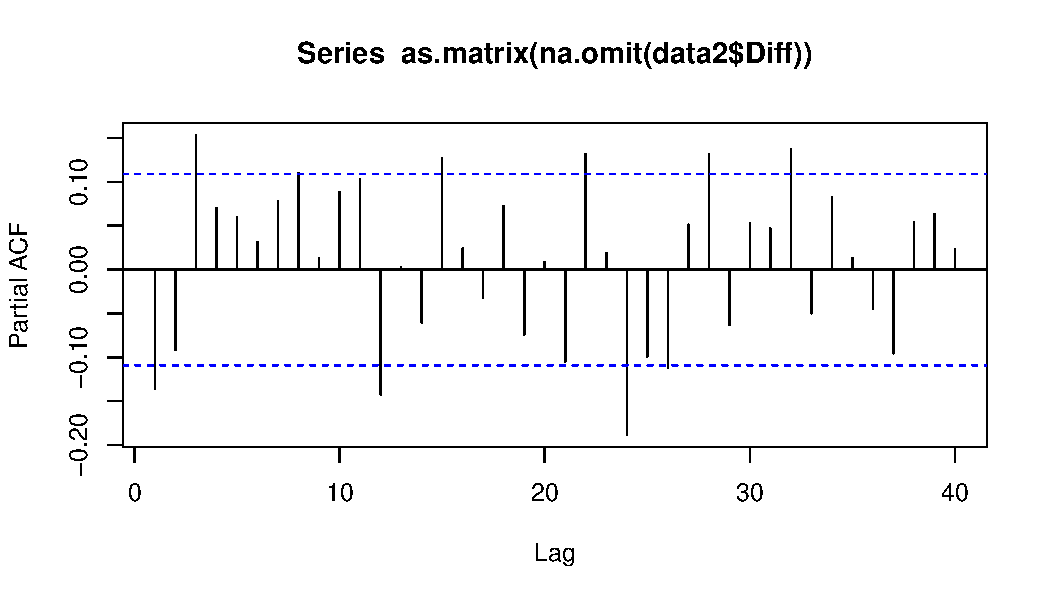
\includegraphics[width=\maxwidth]{figure/unnamed-chunk-86-1} 

\end{knitrout}
            \end{figure}
            
            \begin{figure}[H]
            \caption{FACP dos Resíduos}
            \centering          
\begin{knitrout}
\definecolor{shadecolor}{rgb}{0.969, 0.969, 0.969}\color{fgcolor}\begin{kframe}
\begin{alltt}
\hlkwd{pacf}\hlstd{(}\hlkwd{as.matrix}\hlstd{(model2}\hlopt{$}\hlstd{fit}\hlopt{$}\hlstd{residuals),} \hlkwc{lag.max}\hlstd{=}\hlnum{40}\hlstd{)}
\end{alltt}
\end{kframe}
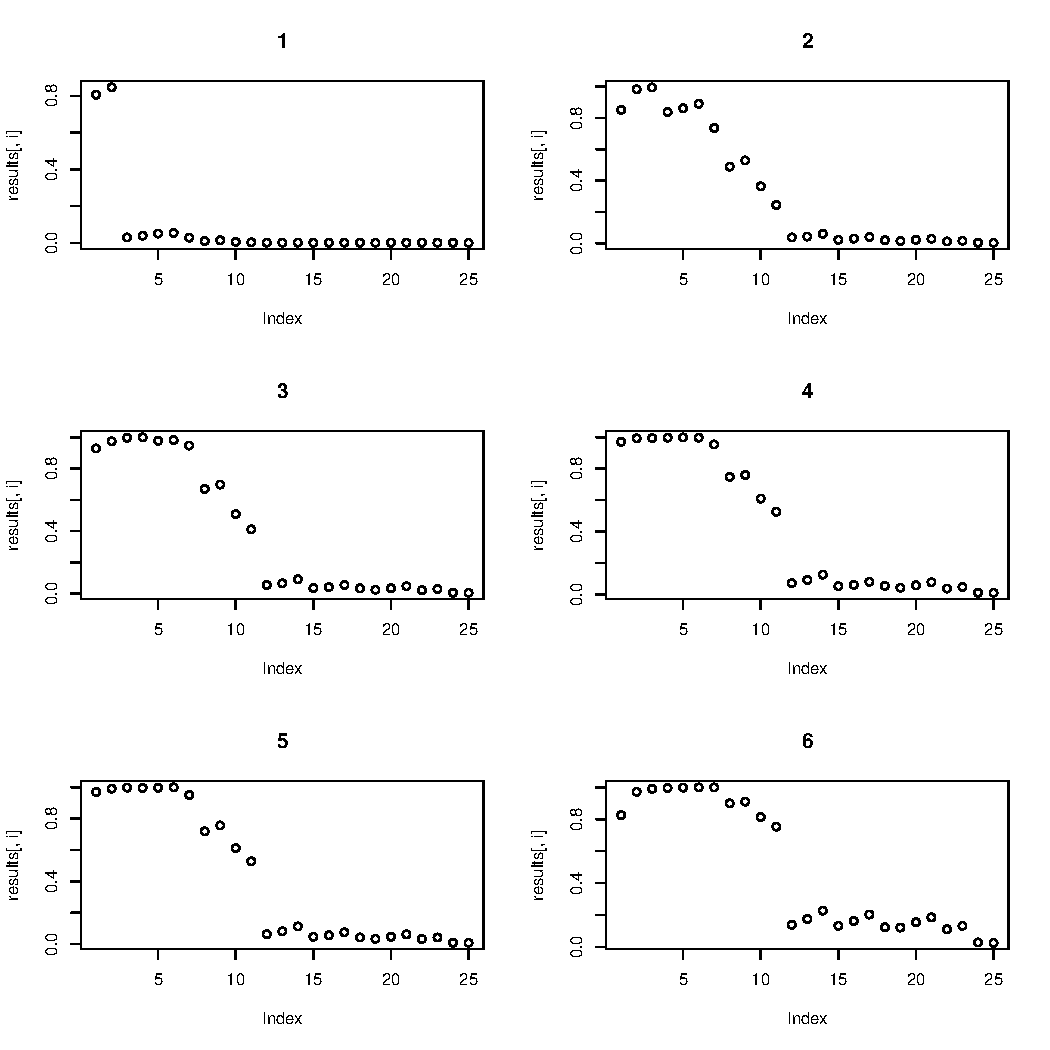
\includegraphics[width=\maxwidth]{figure/unnamed-chunk-87-1} 

\end{knitrout}
            \end{figure}
            
            Tanto o gráfico dos resíduos quanto a sua função de autocorrelação e sua função de autocorrelação parcial indicam que os resíduos se comportam como ruído branco, já que a quantidade de lags significativos é a esperada para um nível de significância de 5\%. o Para testar essa hipótese, realizamos o teste de Ljung-Box para todos os lags até o vinte e cinco. Os testes são realizados no \textit{chunk} abaixo, e na figura abaixo estão os p-valores dos testes para cada lag.
            
\begin{knitrout}
\definecolor{shadecolor}{rgb}{0.969, 0.969, 0.969}\color{fgcolor}\begin{kframe}
\begin{alltt}
\hlstd{boxs} \hlkwb{<-} \hlkwd{all_box}\hlstd{(model2}\hlopt{$}\hlstd{fit}\hlopt{$}\hlstd{residuals)}
\end{alltt}
\end{kframe}
\end{knitrout}

            \begin{figure}[H]
            \caption{P-Valores de Ljung-Box}
            \centering          
\begin{knitrout}
\definecolor{shadecolor}{rgb}{0.969, 0.969, 0.969}\color{fgcolor}\begin{kframe}
\begin{alltt}
\hlkwd{plot}\hlstd{(boxs,} \hlkwc{type}\hlstd{=}\hlstr{'l'}\hlstd{)}
\end{alltt}
\end{kframe}
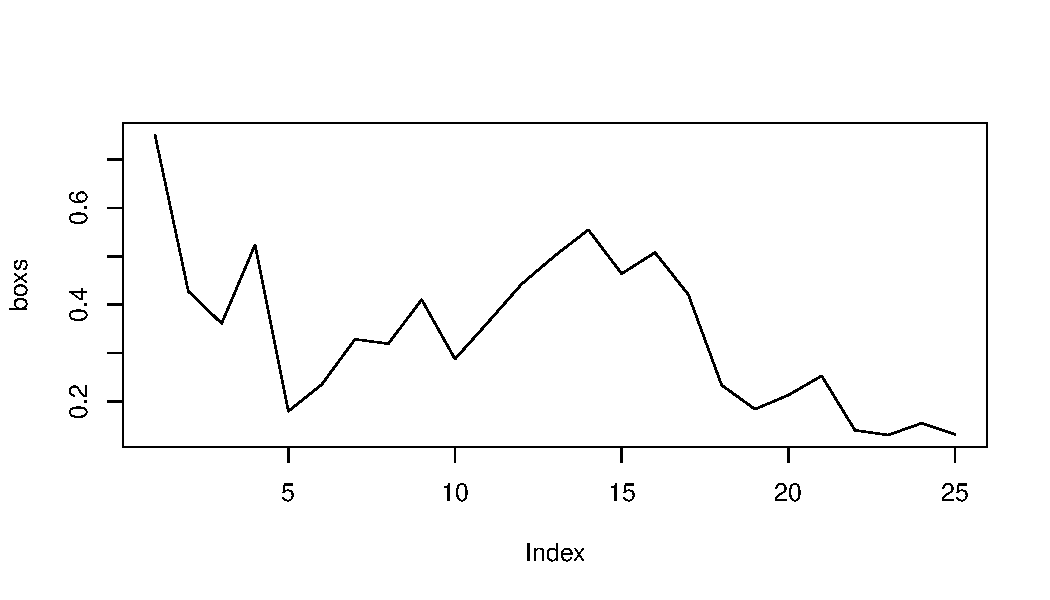
\includegraphics[width=\maxwidth]{figure/unnamed-chunk-89-1} 

\end{knitrout}
            \end{figure}
            
            Abaixo, o valor mínimo do teste de Ljung-Box entre todos os lags considerados.
            
\begin{knitrout}
\definecolor{shadecolor}{rgb}{0.969, 0.969, 0.969}\color{fgcolor}\begin{kframe}
\begin{alltt}
\hlkwd{min}\hlstd{(boxs)}
\end{alltt}
\begin{verbatim}
## [1] 0.1309436
\end{verbatim}
\end{kframe}
\end{knitrout}
            
            Os p-valores não rejeitam a hipótese nula de independência da distribuição, uma vez que todos são superiores a 0,05.
            
        \subsubsection{Homoscedasticidade}
        
            Testamos a homoscedasticidade dos resíduos do modelo selecionado apicando a análise acima nos resíduos ao quadrado.
            
            \begin{figure}[H]
            \caption{Resíduos ao Quadrado}
            \centering
\begin{knitrout}
\definecolor{shadecolor}{rgb}{0.969, 0.969, 0.969}\color{fgcolor}\begin{kframe}
\begin{alltt}
\hlkwd{plot}\hlstd{(model2}\hlopt{$}\hlstd{fit}\hlopt{$}\hlstd{residuals}\hlopt{^}\hlnum{2}\hlstd{)}
\end{alltt}
\end{kframe}
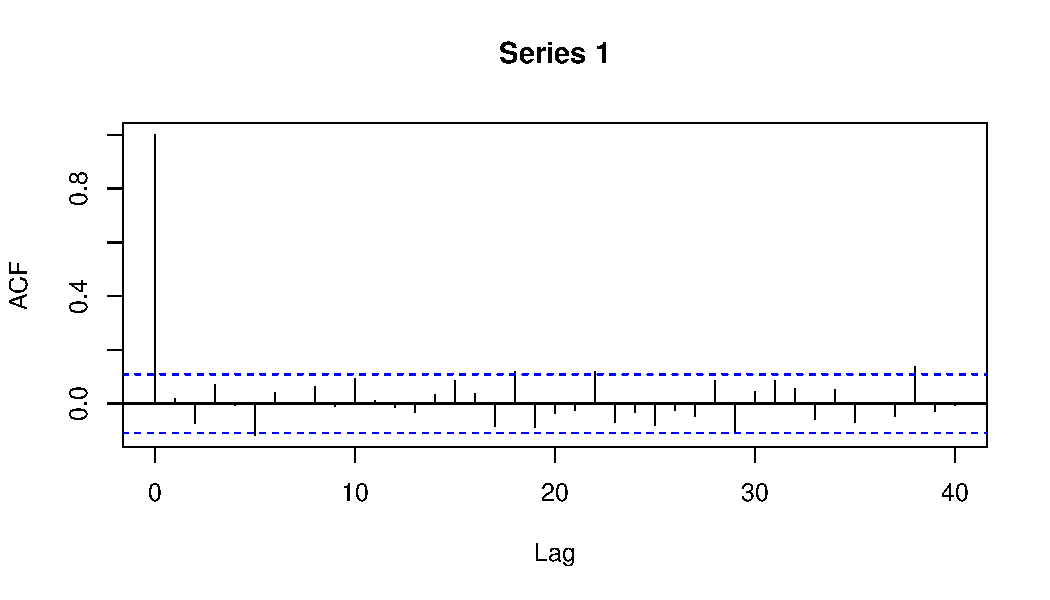
\includegraphics[width=\maxwidth]{figure/unnamed-chunk-91-1} 

\end{knitrout}
            \end{figure}
            
            \begin{figure}[H]
            \caption{FAC dos Resíduos ao Quadrado}
            \centering          
\begin{knitrout}
\definecolor{shadecolor}{rgb}{0.969, 0.969, 0.969}\color{fgcolor}\begin{kframe}
\begin{alltt}
\hlkwd{acf}\hlstd{(}\hlkwd{as.matrix}\hlstd{(model2}\hlopt{$}\hlstd{fit}\hlopt{$}\hlstd{residuals)}\hlopt{^}\hlnum{2}\hlstd{,} \hlkwc{lag.max}\hlstd{=}\hlnum{40}\hlstd{)}
\end{alltt}
\end{kframe}
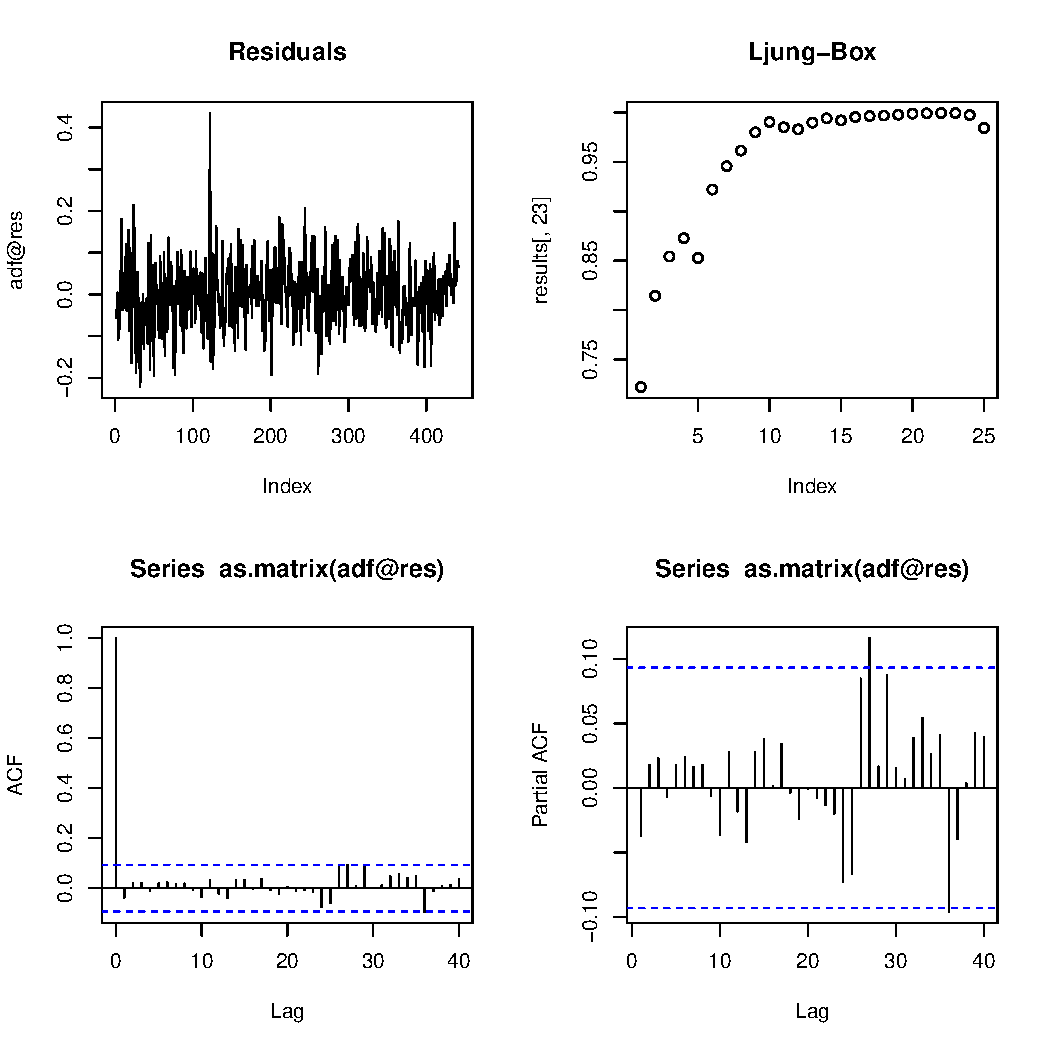
\includegraphics[width=\maxwidth]{figure/unnamed-chunk-92-1} 

\end{knitrout}
            \end{figure}
            
            \begin{figure}[H]
            \caption{FACP dos Resíduos ao Quadrado}
            \centering          
\begin{knitrout}
\definecolor{shadecolor}{rgb}{0.969, 0.969, 0.969}\color{fgcolor}\begin{kframe}
\begin{alltt}
\hlkwd{pacf}\hlstd{(}\hlkwd{as.matrix}\hlstd{(model2}\hlopt{$}\hlstd{fit}\hlopt{$}\hlstd{residuals)}\hlopt{^}\hlnum{2}\hlstd{,} \hlkwc{lag.max}\hlstd{=}\hlnum{40}\hlstd{)}
\end{alltt}
\end{kframe}
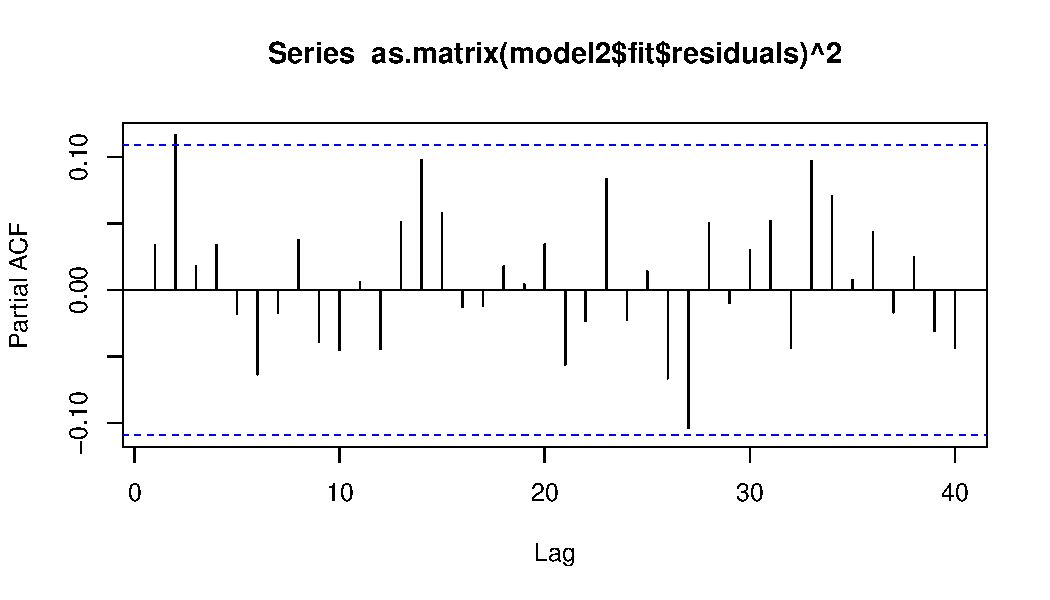
\includegraphics[width=\maxwidth]{figure/unnamed-chunk-93-1} 

\end{knitrout}
            \end{figure}
            
            Tanto o gráfico dos resíduos ao quadrado quanto a sua função de autocorrelação e sua função de autocorrelação parcial indicam homoscedasticidade. Para testar essa hipótese, realizamos o teste de Ljung-Box nos resíduos ao quadrado para todos os lags até o vinte e cinco. Os testes são realizados no \textit{chunk} abaixo, e na figura abaixo estão os p-valores dos testes para cada lag.
            
\begin{knitrout}
\definecolor{shadecolor}{rgb}{0.969, 0.969, 0.969}\color{fgcolor}\begin{kframe}
\begin{alltt}
\hlstd{boxs} \hlkwb{<-} \hlkwd{all_box}\hlstd{(model2}\hlopt{$}\hlstd{fit}\hlopt{$}\hlstd{residuals}\hlopt{^}\hlnum{2}\hlstd{)}
\end{alltt}
\end{kframe}
\end{knitrout}

            \begin{figure}[H]
            \caption{P-Valores de Ljung-Box}
            \centering          
\begin{knitrout}
\definecolor{shadecolor}{rgb}{0.969, 0.969, 0.969}\color{fgcolor}\begin{kframe}
\begin{alltt}
\hlkwd{plot}\hlstd{(boxs,} \hlkwc{type}\hlstd{=}\hlstr{'l'}\hlstd{)}
\end{alltt}
\end{kframe}
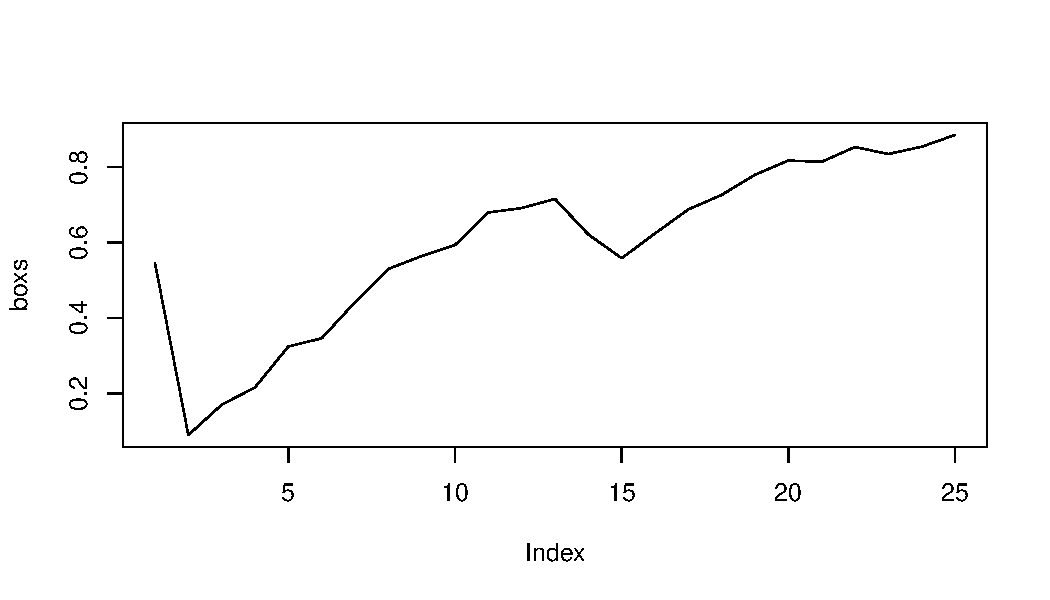
\includegraphics[width=\maxwidth]{figure/unnamed-chunk-95-1} 

\end{knitrout}
            \end{figure}
            
        Abaixo, o valor mínimo do teste de Ljung-Box entre todos os lags considerados.
            
\begin{knitrout}
\definecolor{shadecolor}{rgb}{0.969, 0.969, 0.969}\color{fgcolor}\begin{kframe}
\begin{alltt}
\hlkwd{min}\hlstd{(boxs)}
\end{alltt}
\begin{verbatim}
## [1] 0.08952865
\end{verbatim}
\end{kframe}
\end{knitrout}
            
            Os p-valores não rejeitam a hipótese nula de independência da distribuição. Os resíduos podem ser considerados então homoscedásticos, pois os resíduos ao quadrado são `bem comportados' (ruído branco). Não é necessário então estimar um modelo de variância condicional.


    \subsection{Previsão e Acurácia}
    
        Nesta subseção faremos previsões e testaremos a acurácia das previsões feitas, como passo na avaliação do modelo estimado.
    
        \subsubsection{Previsão}
        
            Agora, realizaremos previsões para os últimos 10 períodos da amostra. Faremos previsão recursiva, ou seja: prevemos sempre apenas o período imediatamente subsequente, utilizando todos os dados até então.
        
\begin{knitrout}
\definecolor{shadecolor}{rgb}{0.969, 0.969, 0.969}\color{fgcolor}\begin{kframe}
\begin{alltt}
\hlstd{fs} \hlkwb{<-} \hlkwd{prediction}\hlstd{(data2}\hlopt{$}\hlstd{Value,}\hlnum{1}\hlstd{,}\hlnum{2}\hlstd{,}\hlnum{0}\hlstd{,}\hlnum{2}\hlstd{)}
\end{alltt}
\end{kframe}
\end{knitrout}

          Abaixo, as previsões realizadas.

\begin{knitrout}
\definecolor{shadecolor}{rgb}{0.969, 0.969, 0.969}\color{fgcolor}\begin{kframe}
\begin{alltt}
\hlstd{fs}
\end{alltt}
\begin{verbatim}
##  [1] 2.160667 1.939964 2.144997 2.180143 2.143683 1.977818 1.831369 2.059727
##  [9] 1.846058 1.647538
\end{verbatim}
\end{kframe}
\end{knitrout}

            Abaixo, os gráficos das previsões e da série original.

            \begin{figure}[H]
            \caption{Previsões e Série Original}
            \centering
\begin{knitrout}
\definecolor{shadecolor}{rgb}{0.969, 0.969, 0.969}\color{fgcolor}\begin{kframe}
\begin{alltt}
\hlstd{length} \hlkwb{<-} \hlkwd{length}\hlstd{(data2}\hlopt{$}\hlstd{Value)}
\hlstd{start}  \hlkwb{<-} \hlstd{length} \hlopt{-} \hlnum{9}
\hlstd{series} \hlkwb{<-} \hlstd{data2}\hlopt{$}\hlstd{Value[start}\hlopt{:}\hlstd{length]}
\hlkwd{par}\hlstd{(}\hlkwc{mfrow} \hlstd{=} \hlkwd{c}\hlstd{(}\hlnum{2}\hlstd{,}\hlnum{1}\hlstd{))}
\hlkwd{plot}\hlstd{(fs,}\hlkwc{type}\hlstd{=}\hlstr{'l'}\hlstd{,} \hlkwc{main}\hlstd{=}\hlstr{'Previsões'}\hlstd{)}
\hlkwd{plot}\hlstd{(series)}
\end{alltt}
\end{kframe}
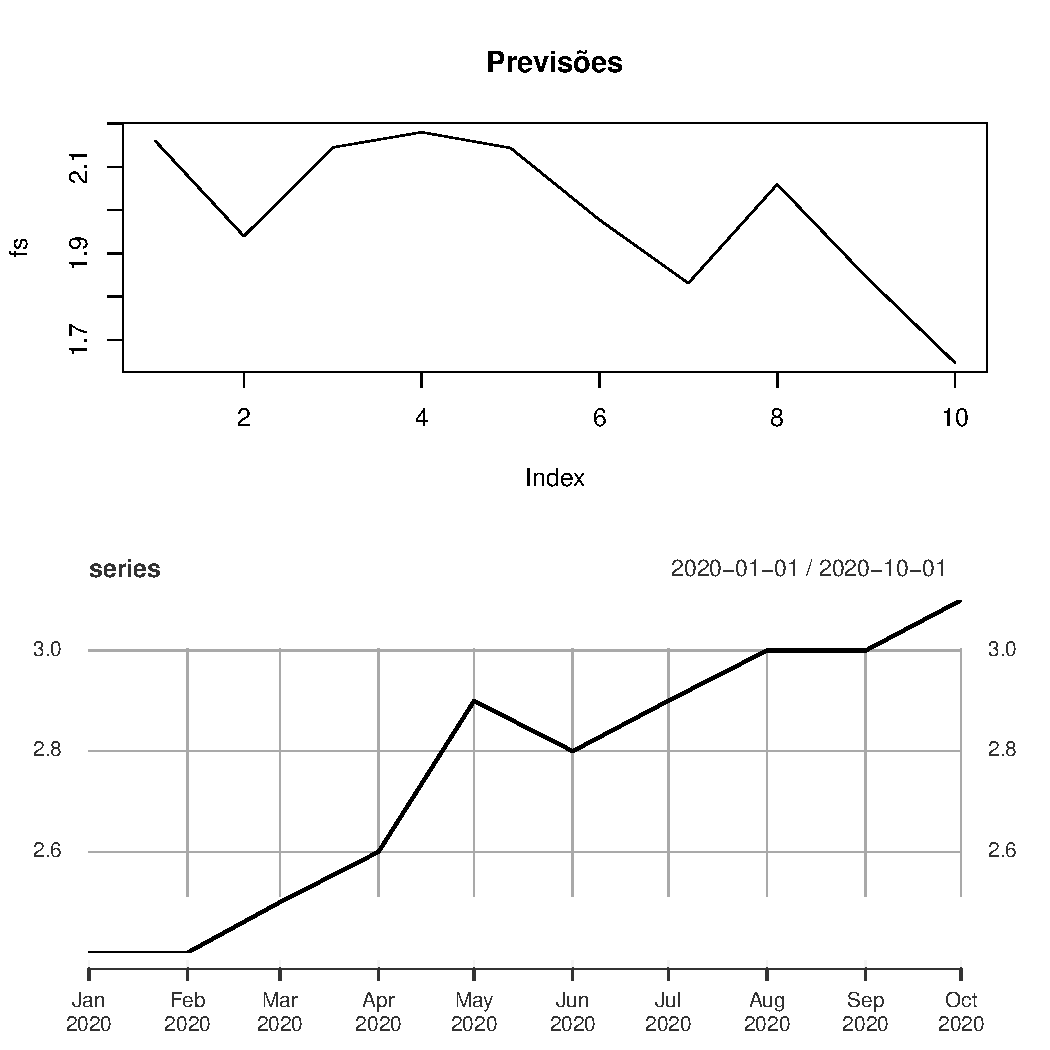
\includegraphics[width=\maxwidth]{figure/unnamed-chunk-98-1} 

\end{knitrout}
            \end{figure}
            
        \subsubsection{Acurácia}

            Agora, vamos calcular a acurácia das previsões. Utilizaremos cinco medidas alternativas: erro médio (ME); erro quadrático médio (RMSE); erro médio absoluto (MAE); erro de porcentagem média (MPE); erro de porcentagem média absoluta (MAPE).
            
\begin{knitrout}
\definecolor{shadecolor}{rgb}{0.969, 0.969, 0.969}\color{fgcolor}\begin{kframe}
\begin{alltt}
\hlkwd{accuracy}\hlstd{(fs,}\hlkwd{as.matrix}\hlstd{(series))}
\end{alltt}
\begin{verbatim}
##                 ME      RMSE       MAE      MPE     MAPE
## Test set 0.7668036 0.8536119 0.7668036 26.84425 26.84425
\end{verbatim}
\end{kframe}
\end{knitrout}

            As medidas acima podem ser úteis na escolha entre modelos, mas não nos dizem muito sobre o modelo se não temos outro para comparar. Para isso usamos o cálculo do Theil's U, que compara as previsões com o que seria uma `adivinhação'. Caso o valor do cálculo for menor que 1, as previsões são melhores que adivinhação. Caso for maior, são piores. O teste é realizado abaixo.
            
\begin{knitrout}
\definecolor{shadecolor}{rgb}{0.969, 0.969, 0.969}\color{fgcolor}\begin{kframe}
\begin{alltt}
\hlkwd{TheilU}\hlstd{(series,fs)}
\end{alltt}
\begin{verbatim}
## [1] 0.3080207
\end{verbatim}
\end{kframe}
\end{knitrout}
            
            O índice do teste foi de 0,308, menor que 1. O modelo fez previsões melhores que uma simples adivinhação.
            
            
            
            
        
        



\section{Conclusão}

    Neste trabalho utilizamos as técnicas apresentadas na disciplina Estatística Econômica Aplicada para analisar uma série temporal. A série original possuía um outlier e uma quebra estrutural, então foram estimados modelos para duas séries temporais diferentes (duas partes da série temporal original). Ambas as séries temporais apresentaram sazonalidade, e não foram necessários modelos de variância condicional. As previsões dos modelos mostraram-se melhores que pura adivinhação, apontando para uma boa qualidade dos modelos.




\printbibliography[heading=bibintoc]

\end{document}
